\chapter{线性方程组的数值求解}\label{ch:2}
\SourcePage{31}

线性代数方程组的求解是科学计算中大多数计算任务的核心.这里介绍几种最常用的、适用于一般形式方程组的方法.更完整的阐述可参见本章各处引用的文献.至于由偏微分方程离散化所产生的方程组,本书会结合具体情形讨论相应的专用技术.

\section{直接法}\label{sec:2.1}

考虑实代数方程组
\begin{equation}\label{eq:2.1.1}
  A\boldsymbol{x}=\boldsymbol{b},
\end{equation}
其中 \(A\) 是一个 \(n\) 阶非奇异矩阵.

若无舍入误差,直接法能在有限步内给出\eqref{eq:2.1.1}的精确解.最经典的直接法是 \emph{Gauss 消去法}(GEM).它将 \(A\) 分解为 \(LU\),其中 \(L\) 是下三角矩阵,\(U\) 是上三角矩阵.这一分解通过下面的过程完成,共得到 \(n\) 个阶段矩阵：
\begin{equation}\label{eq:2.1.2}
  A=A^{(1)}\longrightarrow A^{(2)}\longrightarrow\cdots
  \longrightarrow A^{(n)}=U=L^{-1}A.
\end{equation}
核心思想是,从 \(A^{(k)}\) 到 \(A^{(k+1)}\) 时,对 \(A^{(k)}\) 作变换,使新矩阵 \(A^{(k+1)}\) 第 \(k\) 列中位于对角线下方的元素全部变为零.\figref{fig:2.1.1}示意了这一过程,其中阴影区域表示第 \(k\) 步中发生变化的部分.

相应的算法可简写如下.
\SourcePage{32}

\begin{figure}[htbp]
  \centering
  \includegraphics[page=32,pagebox=cropbox,trim=81.17bp 513.67bp 72.83bp 85.00bp,clip,width=.648\paperwidth]{../input/source/Numerical Approximation of Partial Differential Equations.pdf}
  \caption{Gauss 消去过程}\label{fig:2.1.1}
\end{figure}

\begin{eqalgorithm}\label{eq:2.1.3}
    \ForVar{$k=1,\ldots,n-1$}
        \ForVar{$i=k+1,\ldots,n$}
            \State $m_{ik}=a_{ik}^{(k)}/a_{kk}^{(k)}$
            \ForVar{$j=k+1,\ldots,n$}
                \State $a_{ij}^{(k+1)}
                    =a_{ij}^{(k)}-m_{ik}a_{kj}^{(k)}$
            \EndForVar{$j$}
        \EndForVar{$i$}
    \EndForVar{$k$}
\end{eqalgorithm}
这里,\(a_{ij}^{(1)}\) 是矩阵 \(A=A^{(1)}\) 的元素,而称为\emph{乘子}的 \(m_{ik}\) 是下三角因子 \(L\) 的非对角元素.此外,\(l_{ii}=1\)(\(i=1,\ldots,n\)).这一算法需要 \(O(n^3)\) 次运算.遗憾的是,如果 \(A\) 有一个奇异的顺序主子矩阵,等价地说,如果至少有一个主元 \(a_{kk}^{(k)}\) 为零,算法就可能提前中止.

即使主元始终非零,也可能因主元过小而使 Gauss 消去法不稳定.通常可用选主元策略缓解这一问题.在消去过程的第 \(k\) 步,可在 \(A^{(k)}\) 的第 \(k\) 列至最后一列中交换列(按列交换的部分选主元),也可在第 \(k\) 行至最后一行中交换行(按行交换的部分选主元),还可同时在这一范围内交换行和列(完全选主元),使换到第 \(k\) 个对角位置的新元素 \(\widetilde a_{kk}^{(k)}\) 的绝对值在相应搜索范围内达到最大.\figref{fig:2.1.2}给出了示意图.

\begin{figure}[htbp]
  \centering
  \includegraphics[page=32,pagebox=cropbox,trim=92.50bp 137.00bp 88.83bp 459.00bp,clip,width=.589\paperwidth]{../input/source/Numerical Approximation of Partial Differential Equations.pdf}
  \caption{按列交换的部分选主元(左)、按行交换的部分选主元(中)与完全选主元(右)}\label{fig:2.1.2}
\end{figure}

这相当于将每个 \(A^{(k)}\) 分别从左侧和右侧乘以两个置换矩阵,得到
\[
  \widetilde A^{(k)}=P_k A^{(k)}\Pi_k,
\]
\SourcePage{33}然后直接在 \(\widetilde A^{(k)}\) 上继续消去.整个完全选主元过程给出分解 \(PA\Pi=LU\),其中 \(P\) 和 \(\Pi\) 是置换矩阵.按行交换的部分选主元给出 \(QA=LU\),其中 \(Q\) 是一个置换矩阵；按列交换时则相应得到 \(AQ=LU\).

若将比较前取绝对值也计入,部分选主元的搜索约需 \(n^2\) 次基本操作,而完全选主元的搜索约需 \(2n^3/3\) 次.实际计算中,往往优先采用部分选主元.

这里回顾一下,在不计舍入误差时,如果 \(A\) 是\emph{严格对角占优}的,即
\begin{equation}\label{eq:2.1.4}
  |a_{ii}|>\sum_{\substack{j=1\\j\ne i}}^n|a_{ij}|,\qquad i=1,\ldots,n,
\end{equation}
或者 \(A\) 是一个 \(M\)\emph{-矩阵},即
\begin{equation}\label{eq:2.1.5}
  a_{ij}\le0\quad(i,j=1,\ldots,n,\ i\ne j),
  \qquad (A^{-1})_{ij}\ge0\quad(i,j=1,\ldots,n),
\end{equation}
那么 Gauss 消去法可以在不选主元的情况下进行(例如,见\BookCite{varga1962}{Varga(1962)}第 85 页).

下述结果值得记住(见\BookCite{varga1962}{Varga(1962)}和\BookCite{ortega1988}{Ortega(1988)}).

\begin{lemma}[]{2.1.1}
若 \(A\) 严格对角占优,且对所有 \(i\ne j\) 均有 \(a_{ij}\le0\),对 \(i=1,\ldots,n\) 均有 \(a_{ii}>0\),则 \(A\) 是一个 \(M\)-矩阵.
\end{lemma}

\begin{proof}
将 \(A\) 写成 \(A=D-K\),其中 \(D:=\operatorname{diag}(a_{ii})\) 是以 \(a_{ii}\) 为对角元素的对角矩阵.显然,\(D\) 非奇异,且 \(K_{ij}\ge0\).

由 Gershgorin 圆盘定理(例如,见\BookCite{varga1962}{Varga(1962)}第 16 页)可知,\(D^{-1}K\) 的所有特征值均位于复平面的单位圆内部.因此
\[
  A^{-1}=(I-D^{-1}K)^{-1}D^{-1}
  =\sum_{j=0}^\infty(D^{-1}K)^j D^{-1},
\]
其中 \(I\) 表示单位矩阵.于是 \((A^{-1})_{ij}\ge0\),结论成立.\hfill\(\square\)
\end{proof}

由\eqref{eq:2.1.2}可见,Gauss 消去过程将原矩阵分解为 \(A=LU\).因此,求解\eqref{eq:2.1.1}归结为求解三角方程组 \(L\boldsymbol{y}=\boldsymbol{b}\) 和 \(U\boldsymbol{x}=\boldsymbol{y}\),分别用前代和回代即可完成,所需运算量为 \(O(n^2)\).

还要注意,可以用下列“紧凑”算法直接计算因子 \(L\) 和 \(U\).考虑到 \(l_{kk}=1\)(\(k=1,\ldots,n\)),算法可写成
\SourcePage{34}
\begin{equation}\label{eq:2.1.6}
  \left\{
  \begin{aligned}
    &\text{对 }k=1,\ldots,n\\
    &\quad\text{对 }j=k,\ldots,n\\
    &\qquad u_{kj}=a_{kj}-\sum_{p=1}^{k-1} l_{kp}u_{pj}\\
    &\quad\text{结束 \(j\) 循环}\\
    &\quad\text{若 \(k\ne n\),对 }i=k+1,\ldots,n\\
    &\qquad l_{ik}=\frac1{u_{kk}}\left(a_{ik}-\sum_{p=1}^{k-1} l_{ip}u_{pk}\right)\\
    &\quad\text{结束 \(i\) 循环}\\
    &\text{结束 \(k\) 循环.}
  \end{aligned}
  \right.
\end{equation}
(这里和下文都约定,若求和下限大于上限,则该和取零.此处 \(k=1\) 时就是这种情形.)同样可以用类似算法得到满足 \(u_{kk}=1\) 的分解 \(A=LU\).

若 \(A\) 的所有顺序主子矩阵均非奇异,则存在两个对角元素全为 \(1\) 的下三角矩阵 \(L,M\) 和一个对角矩阵 \(D\),使得
\begin{equation}\label{eq:2.1.7}
  A=LDM^T,
\end{equation}
其中 \(M^T\) 表示矩阵 \(M\) 的转置.有了这一分解,只需依次求解三个具有特殊结构的方程组：
\[
  L\boldsymbol{y}=\boldsymbol{b},\qquad D\boldsymbol{z}=\boldsymbol{y},\qquad M^T\boldsymbol{x}=\boldsymbol{z}.
\]
若 \(A\) 对称,则 \(M=L\),因而\eqref{eq:2.1.7}变为 \(A=LDL^T\).

\begin{definition*}[正定矩阵]
如果方阵 \(A\) 满足
\begin{equation}\label{eq:2.1.8}
  (A\boldsymbol{w},\boldsymbol{w})>0\qquad
  \text{对所有 \(\boldsymbol{w}\in\mathbb R^n\)、\(\boldsymbol{w}\ne\boldsymbol{0}\),}
\end{equation}
则称它是{\heiti 正定的},简记为 \(A>0\).这里 \((\cdot,\cdot)\) 是 \(\mathbb R^n\) 中的 Euclid 内积.
\end{definition*}
请读者注意,有些文献称这一性质为“正实性”(例如,见\BookCite{young1971}{Young(1971)}),并将“正定”一词仅用于对称矩阵.

若 \(A\) 正定且对称,Sylvester 定理保证它的所有顺序主子矩阵均非奇异,并且 \(A\) 有如下 \emph{Cholesky 分解}：
\begin{equation}\label{eq:2.1.9}
  A=LL^T,
\end{equation}
其中 \(L\) 是对角元素为正的下三角矩阵.这一分解唯一.可以用下面的算法求出 \(L\) 的元素,计算时无需选主元：
\SourcePage{35}
\begin{equation}\label{eq:2.1.10}
  \left\{
  \begin{aligned}
    &\text{对 }k=1,\ldots,n\\
    &\quad l_{kk}=\left(a_{kk}-\sum_{p=1}^{k-1}l_{kp}^2\right)^{1/2}\\
    &\quad\text{若 \(k\ne n\),对 }i=k+1,\ldots,n\\
    &\qquad l_{ik}=\frac1{l_{kk}}\left(a_{ik}-\sum_{p=1}^{k-1}l_{ip}l_{kp}\right)\\
    &\quad\text{结束 \(i\) 循环}\\
    &\text{结束 \(k\) 循环.}
  \end{aligned}
  \right.
\end{equation}
这一算法需要 \(O(n^3)\) 次运算,约为完整 Gauss 消去过程所需运算量的一半,此外还需要 \(n\) 次开平方.

若 \(A\) 是对称不定矩阵,适当选主元后仍可作 \(LDL^T\) 型分解.直接计算时,因子中的元素可能变得任意大.为了避免这一问题,必须采用某种选主元策略.Bunch 和 Kaufman 的算法以及 Aasen 的算法都可高效地做到这一点,计算 \(LDL^T\) 型分解所需的运算量仍为 \(O(n^3)\).有关介绍见\BookCite{golub-vanloan1989}{Golub 和 Van Loan(1989)}第 4.4 节,亦可参见\BookCite{barwell-george1976}{Barwell 和 George(1976)}.

对于一般矩阵 \(A\),还有另一种分解,称为 \emph{\(QR\) 分解}.它的计算代价比 \(LU\) 分解高,但更稳定.对于任意秩为 \(n\) 的实矩阵 \(A\in\mathbb R^{m\times n}\)(有 \(m\) 行和 \(n\) 列,且 \(m\ge n\)),存在唯一的矩阵 \(Q\in\mathbb R^{m\times n}\) 满足
\begin{equation}\label{eq:2.1.11}
  Q^TQ=D,\qquad D=\operatorname{diag}(d_1,\ldots,d_n),\qquad
  d_k>0\quad(k=1,\ldots,n),
\end{equation}
以及一个满足 \(r_{kk}=1\)(\(k=1,\ldots,n\))的上三角矩阵 \(R\in\mathbb R^{n\times n}\),使得
\begin{equation}\label{eq:2.1.12}
  A=QR.
\end{equation}

这种分解特别适合求解\emph{最小二乘问题}.事实上,由\eqref{eq:2.1.12}可知,\emph{正规方程}
\begin{equation}\label{eq:2.1.13}
  A^TA\boldsymbol{x}=A^T\boldsymbol{b}
\end{equation}
可写成
\[
  0=A^T(\boldsymbol{b}-A\boldsymbol{x})=R^TQ^T(\boldsymbol{b}-A\boldsymbol{x})
    =R^T(Q^T\boldsymbol{b}-Q^TQR\boldsymbol{x}),
\]
于是
\begin{equation}\label{eq:2.1.14}
  D\boldsymbol{y}=Q^T\boldsymbol{b},\qquad R\boldsymbol{x}=\boldsymbol{y}.
\end{equation}
因此,求\eqref{eq:2.1.13}的解只需解两个方程组,一个是对角方程组,另一个是上三角方程组.

因子 \(Q\) 和 \(R\) 可用多种算法计算.一种基于修正的 Gram--Schmidt 正交化方法；另一种是 Householder 法,使用反射矩阵；\SourcePage{36}第三种是 Givens 法,使用旋转矩阵,所需运算量是 Householder 法的两倍(例如,见\BookCite{isaacson-keller1966}{Isaacson 和 Keller(1966)}以及\BookCite{golub-vanloan1989}{Golub 和 Van Loan(1989)}).

\subsection{带状方程组}\label{sec:2.1.1}

在许多实际情形中,若方程组\eqref{eq:2.1.1}来自微分问题的离散化,则矩阵 \(A\) 为带状矩阵.也就是说,存在整数 \(q\)(带宽),\(1\le q<n\),使得
\begin{equation}\label{eq:2.1.15}
  a_{ij}=0\qquad \text{当 }|i-j|>q\text{ 时.}
\end{equation}
特别地,\(A\) 的每一行至多有 \(2q+1\) 个非零元素.

求解带状方程组时,\(A\) 的三角因子也可以保持带状,从而显著节省存储空间和运算量.事实上,如果 \(A\) 的带宽为 \(q\),并且可以直接作 \(LU\) 分解,则两个三角因子 \(L\) 和 \(U\) 都是带宽为 \(q\) 的带状矩阵.Gauss 消去算法\eqref{eq:2.1.3}只需稍作修改,所需运算量为 \(O(nq^2)\).相应的三角方程组用前代或回代求解时,需要 \(O(nq)\) 次运算.

一般来说,如果在 Gauss 消去法中采用选主元策略,所得因子未必保持 \(A\) 原来的带状结构.具体而言,\(U\) 的带宽可以大于 \(A\) 的上三角部分的带宽(按行作部分选主元时,\(U\) 的带宽至多为 \(2q\)).对 \(L\) 的带宽,一般甚至无法给出相应的界,不过可以证明,按行作部分选主元时,\(L\) 每列至多有 \(q+1\) 个非零元素.

若 \(A\) 对称、正定且满足\eqref{eq:2.1.15},则其 Cholesky 分解\eqref{eq:2.1.9}可按下列算法计算：
\begin{equation}\label{eq:2.1.16}
  \left\{
  \begin{aligned}
    &\text{对 }k=1,\ldots,n\\
    &\quad s_k=\max(1,k-q),\qquad r_k=\min(n,k+q)\\
    &\quad l_{kk}=\left(a_{kk}-\sum_{p=s_k}^{k-1}l_{kp}^2\right)^{1/2}\\
    &\quad\text{若 \(k\ne n\),对 }i=k+1,\ldots,r_k\\
    &\qquad l_{ik}=\frac1{l_{kk}}\left(a_{ik}-\sum_{p=s_i}^{k-1}l_{ip}l_{kp}\right)\\
    &\quad\text{结束 \(i\) 循环}\\
    &\text{结束 \(k\) 循环.}
  \end{aligned}
  \right.
\end{equation}
这一算法需要 \(O(nq^2)\) 次运算,约为完整 Gauss 消去法所需运算量的一半,此外还需要 \(n\) 次开平方.

\begin{note}\NumberedNote{note:2.1.1}{\heiti(稀疏方程组)}
如果 \(A\) 的带宽 \(q\) 远小于它的阶数 \(n\),那么 \(A\) 是稀疏的.更一般地,若 \(A\) 的非零元素个数为 \(O(n)\),则称 \(A\) 为稀疏矩阵.

\SourcePage{37}
稀疏矩阵与带状矩阵不同,它的拓扑结构往往并不明确.例如,当偏微分方程在非结构网格上离散,或网格点编号不当时,所得方程组就可能具有这种性质.

用于求解稀疏方程组的直接法,应当能够利用 \(A\) 的稀疏性.事实上,如果对稀疏矩阵作分解时不顾及它的结构,就可能出现大量{\heiti 填充},也就是产生相当多的新非零元素.

可以按特定准则重排行和列来减少填充.对于偏微分方程,这等同于给节点重新编号.这类方法包括嵌套剖分法及其变体.

另一种做法是巧妙地利用数据结构.有关求解稀疏方程组的专用直接法的分析,参见\BookCite{bunch-rose1976}{Bunch 和 Rose(1976)}、\BookCite{bjorck-plemmons-schneider1981}{Björck、Plemmons 和 Schneider(1981)}、\BookCite{george-liu1981}{George 和 Liu(1981)}以及\BookCite{duff-erisman-reid1986}{Duff、Erisman 和 Reid(1986)}.\hfill\(\square\)
\end{note}

\begin{note}\NumberedNote{note:2.1.2}{\heiti(专用技术)}
在特定情形下,可以用专门的方式实现 Gauss 消去法.我们将在第~\BookRef{sec:6.3.2}{6.3.2}~节讨论其中一些方法.这里列出三个值得注意的例子：
\begin{enumerate}[label=(\roman*),leftmargin=*]
  \item {\heiti 波前法},即按适当顺序对有限元刚度矩阵作 Gauss 消去,见\BookCite{liu1992}{Liu(1992)}的综述.
  \item {\heiti 快速 Poisson 求解器},用于在结构网格上离散 Poisson 方程所得到的有限元(或有限差分)方程组,见\BookCite{buzbee-golub-nielson1970}{Buzbee、Golub 和 Nielson(1970)}及\BookCite{dorr1970}{Dorr(1970)},另见\BookCite{vajtersic1993}{Vajteršič(1993)}.
  \item Haidvogel--Zang 对角化,用于 Poisson 问题的谱 Galerkin 逼近所对应的矩阵,见\BookCite{haidvogel-zang1979}{Haidvogel 和 Zang(1979)},也用于 Helmholtz 方程的谱配置逼近所对应的矩阵,见\BookCite{haldenwang-labrosse-abboudi-deville1984}{Haldenwang、Labrosse、Abboudi 和 Deville(1984)}.\hfill\(\square\)
\end{enumerate}
\end{note}

\subsection{误差分析}\label{sec:2.1.2}

先回顾几个关于矩阵的基本概念和记号.
\begin{definition*}[矩阵范数]
矩阵范数是函数 \(f\colon\mathbb R^{n\times n}\to\mathbb R\),对任意 \(A,B\in\mathbb R^{n\times n}\),满足
\[
  \begin{aligned}
    f(A)&\ge0\quad\text{(\(f(A)=0\) 当且仅当 \(A=0\))},\\
    f(A+B)&\le f(A)+f(B),\\
    f(\alpha A)&=|\alpha|f(A),\qquad \alpha\in\mathbb R,\\
    f(AB)&\le f(A)f(B).
  \end{aligned}
\]
\end{definition*}
矩阵范数通常用带下标的双竖线表示,即 \(\|A\|=f(A)\).

Frobenius 范数
\SourcePage{38}
\begin{equation}\label{eq:2.1.17}
  \|A\|_F:=\left(\sum_{i,j=1}^n|a_{ij}|^2\right)^{1/2}
\end{equation}
和 \(p\)-范数
\begin{equation}\label{eq:2.1.18}
  \|A\|_p:=\max_{|\boldsymbol{w}|_p=1}|A\boldsymbol{w}|_p,\qquad 1\le p\le\infty,
\end{equation}
是数值线性代数中最常用的矩阵范数.回顾一下,\(\mathbb R^n\) 中向量的 \(p\)-范数定义为
\begin{equation}\label{eq:2.1.19}
  |\boldsymbol{w}|_p:=\left(\sum_{j=1}^n|w_j|^p\right)^{1/p},
  \qquad 1\le p<\infty,
\end{equation}
以及
\begin{equation}\label{eq:2.1.20}
  |\boldsymbol{w}|_\infty:=\max_{1\le j\le n}|w_j|.
\end{equation}

更一般地,对 \(\mathbb R^n\) 中任一向量范数 \(|\cdot|\),可定义与之相应的\emph{诱导矩阵范数}
\[
  \|A\|:=\max_{|\boldsymbol{w}|=1}|A\boldsymbol{w}|.
\]

\begin{definition*}[谱半径]
以 \(\lambda_i(A)\)(\(i=1,\ldots,n\))表示 \(A\) 的特征值,则 \(A\) 的谱半径定义为
\begin{equation}\label{eq:2.1.21}
  \rho(A):=\max\bigl\{|\lambda_i(A)|\mid i=1,\ldots,n\bigr\}.
\end{equation}
\end{definition*}
可以证明,\(\rho(A)\) 是 \(\|A\|\) 取遍所有诱导矩阵范数时的下确界(例如,见\BookCite{isaacson-keller1966}{Isaacson 和 Keller(1966)}第 14 页).

注意,
\begin{equation}\label{eq:2.1.22}
  \|A\|_1=\max_{1\le j\le n}\sum_{i=1}^n|a_{ij}|,
  \qquad
  \|A\|_\infty=\max_{1\le i\le n}\sum_{j=1}^n|a_{ij}|.
\end{equation}
此外,还可作如下刻画(例如,见\BookCite{varga1962}{Varga(1962)}第 11 页)：
\begin{equation}\label{eq:2.1.23}
  \|A\|_2=\sqrt{\rho(A^TA)}=\sqrt{\lambda_{\max}(A^TA)}.
\end{equation}
因此
\begin{equation}\label{eq:2.1.24}
  \|A\|_2=\rho(A)\qquad\text{当 \(A\) 对称时.}
\end{equation}

\begin{definition*}[条件数]
对任意矩阵范数 \(\|\cdot\|\),非奇异矩阵 \(A\) 关于这一范数的条件数是实数
\begin{equation}\label{eq:2.1.25}
  \chi(A):=\|A\|\|A^{-1}\|.
\end{equation}
\end{definition*}

\SourcePage{39}
若 \(\|\cdot\|\) 是诱导矩阵范数,则 \(\chi(A)\ge1\).特别地,以 \(\chi_p(A)\) 表示用\eqref{eq:2.1.18}中的范数计算得到的 \(A\) 的条件数.由\eqref{eq:2.1.23}可得
\begin{equation}\label{eq:2.1.26}
  \chi_2(A)=\sqrt{\frac{\lambda_{\max}(A^TA)}{\lambda_{\min}(A^TA)}}.
\end{equation}
我们进一步定义
\begin{equation}\label{eq:2.1.27}
  \chi_{\mathrm{sp}}(A):=
  \frac{\max\bigl\{|\lambda_i(A)|\mid i=1,\ldots,n\bigr\}}
       {\min\bigl\{|\lambda_i(A)|\mid i=1,\ldots,n\bigr\}}.
\end{equation}
显然,若 \(A\) 对称,则 \(\chi_2(A)=\chi_{\mathrm{sp}}(A)\).为方便起见,即使 \(A\) 不对称,我们也将 \(\chi_{\mathrm{sp}}(A)\) 称为矩阵 \(A\) 的\emph{谱条件数}.关于形如 \(P^{-1}A\) 的矩阵的谱条件数,还可参见引理~\BookRef{lem:2.4.1}{2.4.1}中的一个有用刻画.

如果矩阵的条件数不“大”,便称该矩阵的条件良好,否则称其为病态矩阵.后一种情况下,线性方程组\eqref{eq:2.1.1}的求解可能对扰动非常敏感,因为数据的微小变化就可能导致解发生很大变化.

条件数衡量矩阵的病态程度.为使这一点更明确,设\eqref{eq:2.1.1}中的数据 \(A\) 和 \(\boldsymbol{b}\) 分别受到矩阵 \(E\) 和向量 \(\boldsymbol{e}\) 的扰动.若 \(\overline{\boldsymbol{x}}\) 表示扰动后的方程组
\begin{equation}\label{eq:2.1.28}
  (A+E)\overline{\boldsymbol{x}}=\boldsymbol{b}+\boldsymbol{e}
\end{equation}
的解,则下列结果给出了 \(\overline{\boldsymbol{x}}-\boldsymbol{x}\) 的一个估计.

\begin{proposition}[]{2.1.1}
设 \(A\) 非奇异,\(\boldsymbol{b}\ne\boldsymbol{0}\).对于由向量范数 \(|\cdot|\) 诱导的给定矩阵范数 \(\|\cdot\|\),假定
\begin{equation}\label{eq:2.1.29}
  \|E\|<\frac1{\|A^{-1}\|}.
\end{equation}
若 \(\boldsymbol{x}\) 和 \(\overline{\boldsymbol{x}}\) 分别满足\eqref{eq:2.1.1}和\eqref{eq:2.1.28},则
\begin{equation}\label{eq:2.1.30}
  \frac{|\overline{\boldsymbol{x}}-\boldsymbol{x}|}{|\boldsymbol{x}|}
  \le\frac{\chi(A)}{1-\|A^{-1}\|\|E\|}
  \left(\frac{|\boldsymbol{e}|}{|\boldsymbol{b}|}+\frac{\|E\|}{\|A\|}\right).
\end{equation}
\end{proposition}

\begin{proof}
若矩阵 \(B\) 满足 \(\|B\|<1\),则 \(I-B\) 非奇异,且
\[
  \|(I-B)^{-1}\|\le(1-\|B\|)^{-1}
\]
(例如,见\BookCite{isaacson-keller1966}{Isaacson 和 Keller(1966)}第 16 页).由于 \(\|A^{-1}E\|\le\|A^{-1}\|\|E\|<1\),取 \(B=-A^{-1}E\) 可得
\SourcePage{40}
\begin{equation}\label{eq:2.1.31}
  \|(I+A^{-1}E)^{-1}\|\le\frac1{1-\|A^{-1}\|\|E\|}.
\end{equation}
用\eqref{eq:2.1.28}减去\eqref{eq:2.1.1},得到
\((A+E)(\overline{\boldsymbol{x}}-\boldsymbol{x})=\boldsymbol{e}-E\boldsymbol{x}\).再在等式两边左乘 \(A^{-1}\) 并求解,得到
\[
  \overline{\boldsymbol{x}}-\boldsymbol{x}=(I+A^{-1}E)^{-1}A^{-1}(\boldsymbol{e}-E\boldsymbol{x}).
\]
对等式两边取范数,应用\eqref{eq:2.1.31},再除以 \(|\boldsymbol{x}|\),可得
\[
  \frac{|\overline{\boldsymbol{x}}-\boldsymbol{x}|}{|\boldsymbol{x}|}
  \le\frac{\|A^{-1}\|}{1-\|A^{-1}\|\|E\|}
  \left(\frac{|\boldsymbol{e}|}{|\boldsymbol{x}|}+\|E\|\right).
\]
由\eqref{eq:2.1.1}可知
\[
  |\boldsymbol{x}|\ge\frac{|\boldsymbol{b}|}{\|A\|},
\]
所以可用这个下界替换右端的 \(|\boldsymbol{x}|\).再应用定义\eqref{eq:2.1.25},即得结论\eqref{eq:2.1.30}.\hfill\(\square\)
\end{proof}

\section{迭代法概述}\label{sec:2.2}

迭代法把方程组\eqref{eq:2.1.1}的解表示为序列 \(\{\boldsymbol{x}^k\}\) 的极限.计算中通常只需要用矩阵 \(A\) 与给定向量相乘.大规模稀疏问题是采用迭代法的典型情形.对于带状矩阵,如果带内本身也很稀疏,分解算法就难以实现,这时也会采用迭代法.

一般来说,迭代法以矩阵 \(A\) 的一个适当分裂为基础：
\begin{equation}\label{eq:2.2.1}
  A=P-N,\qquad P\text{ 非奇异.}
\end{equation}
给定 \(\boldsymbol{x}^0\),按下式生成序列 \(\{\boldsymbol{x}^k\}\)：
\begin{equation}\label{eq:2.2.2}
  P\boldsymbol{x}^{k+1}=N\boldsymbol{x}^k+\boldsymbol{b},\qquad k\ge0.
\end{equation}

评价一种迭代法主要看两点：迭代量 \(\boldsymbol{x}^k\) 收敛得有多快,以及每一步求解线性方程组\eqref{eq:2.2.2}的计算代价有多低.先看第一点.令
\begin{equation}\label{eq:2.2.3}
  \boldsymbol{e}^k:=\boldsymbol{x}^k-\boldsymbol{x},\qquad B:=P^{-1}N,
\end{equation}
由\eqref{eq:2.2.2}可得误差方程
\begin{equation}\label{eq:2.2.4}
  \boldsymbol{e}^k=B\boldsymbol{e}^{k-1}=B^k\boldsymbol{e}^0,
\end{equation}
其中 \(\boldsymbol{e}^0\) 是初始误差.

\SourcePage{41}
对任意初始向量 \(\boldsymbol{x}^0\),迭代量 \(\boldsymbol{x}^k\) 收敛到\eqref{eq:2.1.1}的解 \(\boldsymbol{x}\),当且仅当\emph{迭代矩阵} \(B\) 的谱半径满足
\begin{equation}\label{eq:2.2.5}
  \rho(B)<1.
\end{equation}
事实上,对每个 \(\varepsilon>0\),都能找到一个诱导矩阵范数 \(\|\cdot\|_*\),使得 \(\|B\|_*\le\rho(B)+\varepsilon\).由\eqref{eq:2.2.4}可得
\[
  |\boldsymbol{e}^k|_*\le[\rho(B)+\varepsilon]^k|\boldsymbol{e}^0|_*.
\]
取足够小的 \(\varepsilon\),即可得出收敛性.反过来,若 \(\rho(B)\ge1\),可在复化空间中选取初始向量 \(\boldsymbol{x}^0\),使 \(\boldsymbol{e}^0=\boldsymbol{w}^*\),其中 \(\boldsymbol{w}^*\) 是绝对值最大的特征值 \(\lambda_*\) 所对应的特征向量.对这样的初值,\eqref{eq:2.2.4}给出
\[
  |\boldsymbol{e}^k|=|B^k\boldsymbol{e}^0|=|\lambda_*|^k|\boldsymbol{e}^0|
    =[\rho(B)]^k|\boldsymbol{e}^0|.
\]
因此,无论选用哪个向量范数 \(|\cdot|\),误差都不能趋于零.若 \(\boldsymbol{w}^*\) 不是实向量,它的实部和虚部所产生的误差不可能都趋于零,故对实初值的收敛性也不成立.显然,\(\rho(B)\) 越小,迭代的渐近收敛越快.

在 \(B\) 可对角化的特殊情形下,存在非奇异矩阵 \(T\),使得
\[
  B=T\Lambda T^{-1},
\]
其中 \(\Lambda:=\operatorname{diag}(\lambda_1,\ldots,\lambda_n)\),\(\lambda_j\) 是 \(B\) 的特征值.由递推关系\eqref{eq:2.2.4}得到
\[
  \boldsymbol{e}^k=T\Lambda^kT^{-1}\boldsymbol{e}^0.
\]
定义 \(\boldsymbol{\epsilon}^k:=T^{-1}\boldsymbol{e}^k\),立即得到
\[
  \boldsymbol{\epsilon}^k=\Lambda^k\boldsymbol{\epsilon}^0,
\]
即 \(\epsilon^k_j=(\lambda_j)^k\epsilon^0_j\)(\(j=1,\ldots,n\),\(k\ge0\)).因此,在变换后的基下,每次迭代都把误差的第 \(j\) 个分量乘以相应的特征值 \(\lambda_j\),从而使该分量按这个因子衰减(在 \(|\lambda_j|<1\) 时).

由于 \(\Lambda\) 是对角矩阵,对每个 \(1\le p\le\infty\),都有 \(\|\Lambda\|_p=\rho(\Lambda)=\rho(B)\).因此
\[
  |\boldsymbol{e}^k|_p\le\chi_p(T)[\rho(B)]^k|\boldsymbol{e}^0|_p,
  \qquad
  |\boldsymbol{\epsilon}^k|_p\le[\rho(B)]^k|\boldsymbol{\epsilon}^0|_p,
\]
其中 \(\chi_p(T):=\|T\|_p\|T^{-1}\|_p\) 是对角化矩阵 \(T\) 的 \(p\)-条件数.

数 \(\sigma:=-\log\rho(B)\) 称为迭代过程\eqref{eq:2.2.2}的\emph{渐近收敛率}.其倒数 \(1/\sigma\) 可用来衡量初始误差的范数减至原来的 \(1/e\) 时平均需要的迭代步数.

下面给出一些收敛的充分条件.若对所有 \(i,j=1,\ldots,n\),均有 \((P^{-1})_{ij}\ge0\) 和 \(N_{ij}\ge0\),则称分裂\eqref{eq:2.2.1}是\emph{正则的}.

\SourcePage{42}
由关于非负矩阵的 Perron--Frobenius 理论可证,如果\eqref{eq:2.2.1}是正则分裂,且对 \(i,j=1,\ldots,n\) 均有 \((A^{-1})_{ij}\ge0\),则 \(\rho(P^{-1}N)<1\)(\BookCite{varga1962}{Varga(1962)},第 89 页).下述结果可用于比较正则分裂(\BookCite{varga1962}{Varga(1962)},第 90 页).

\begin{theorem}[]{2.2.1}
设 \(A\) 满足 \((A^{-1})_{ij}>0\)(\(i,j=1,\ldots,n\)).考虑 \(A\) 的两个正则分裂 \(A=P_1-N_1\) 和 \(A=P_2-N_2\).进一步假设
\begin{equation}\label{eq:2.2.6}
  (N_2)_{ij}\ge(N_1)_{ij},\qquad i,j=1,\ldots,n,
\end{equation}
且 \(N_2-N_1\) 不是零矩阵,则
\begin{equation}\label{eq:2.2.7}
  \rho(P_1^{-1}N_1)<\rho(P_2^{-1}N_2)<1.
\end{equation}
\end{theorem}

不等式\eqref{eq:2.2.7}说明,只要\eqref{eq:2.2.6}成立,第一个分裂在渐近收敛速度上就优于第二个分裂.注意,条件\eqref{eq:2.2.6}相当容易核验.下面是另一个值得注意的结果.

\begin{theorem}[Householder--John]{2.2.2}
设 \(A\) 是对称正定矩阵,并按\eqref{eq:2.2.1}分裂.若矩阵 \(P+P^T-A\) 正定,则 \(\rho(P^{-1}N)<1\).
\end{theorem}

\begin{proof}
写成 \(P^{-1}N=I-P^{-1}A\).设 \(\lambda\in\mathbb C\) 是 \(I-P^{-1}A\) 的特征值,\(\boldsymbol{z}\in\mathbb C^n\)、\(\boldsymbol{z}\ne\boldsymbol{0}\) 是相应的特征向量.于是
\begin{equation}\label{eq:2.2.8}
  (1-\lambda)P\boldsymbol{z}=A\boldsymbol{z}.
\end{equation}
特别地,由此可知 \(\lambda\ne1\).令 \(\boldsymbol{z}=\boldsymbol{w}+i\boldsymbol{y}\),其中 \(\boldsymbol{w},\boldsymbol{y}\in\mathbb R^n\).对\eqref{eq:2.2.8}两边分别与 \(\boldsymbol{z}\) 作 \(\mathbb C^n\) 中的内积,再考虑所得等式的复共轭.由于 \(A=A^T\),有 \((A\boldsymbol{z},\boldsymbol{z})_{\mathbb C^n}\in\mathbb R\),并且
\[
  (A\boldsymbol{z},\boldsymbol{z})_{\mathbb C^n}
  =(1-\lambda)(P\boldsymbol{z},\boldsymbol{z})_{\mathbb C^n}
  =(1-\overline\lambda)(P^T\boldsymbol{z},\boldsymbol{z})_{\mathbb C^n}.
\]
于是
\begin{equation}\label{eq:2.2.9}
  \left(\frac1{1-\lambda}+\frac1{1-\overline\lambda}-1\right)
  (A\boldsymbol{z},\boldsymbol{z})_{\mathbb C^n}
  =((P+P^T-A)\boldsymbol{z},\boldsymbol{z})_{\mathbb C^n}.
\end{equation}
取\eqref{eq:2.2.9}的实部,容易得到
\[
  \begin{aligned}
    \frac{1-|\lambda|^2}{|1-\lambda|^2}
     [(A\boldsymbol{w},\boldsymbol{w})+(A\boldsymbol{y},\boldsymbol{y})]
    ={}&((P+P^T-A)\boldsymbol{w},\boldsymbol{w})\\
      &+((P+P^T-A)\boldsymbol{y},\boldsymbol{y}),
  \end{aligned}
\]
其中 \((\cdot,\cdot)\) 是 \(\mathbb R^n\) 中的内积.由于 \(A\) 和 \(P+P^T-A\) 都正定,可得 \(|\lambda|<1\),即 \(\rho(P^{-1}N)<1\).\hfill\(\square\)
\end{proof}

\SourcePage{43}
本节最后给出另一个收敛定理.先回顾,若一个矩阵的全部特征值的实部均为正,则称该矩阵是 \(N\)-稳定的(也称负稳定,见\BookCite{young1971}{Young(1971)}).

\begin{theorem}[]{2.2.3}
收敛条件\eqref{eq:2.2.5}成立,当且仅当 \(I-B\) 非奇异,且
\begin{equation}\label{eq:2.2.10}
  H:=(I-B)^{-1}(I+B)\qquad \text{是 \(N\)-稳定的.}
\end{equation}
\end{theorem}

\begin{proof}
假定 \(I-B\) 非奇异,由\eqref{eq:2.2.10}有 \(H+I=2(I-B)^{-1}\) 和 \(H-I=2(I-B)^{-1}B\),故
\[
  B=(H+I)^{-1}(H-I).
\]
若 \(\lambda\) 是 \(B\) 的特征值,则 \(\mu=(1+\lambda)/(1-\lambda)\) 是 \(H\) 的特征值.此外,可写成
\[
  \lambda=\frac{\mu-1}{\mu+1}
    =\frac{(\operatorname{Re}\mu-1)+i\operatorname{Im}\mu}
           {(\operatorname{Re}\mu+1)+i\operatorname{Im}\mu}.
\]
所以 \(|\lambda|<1\) 当且仅当 \(\operatorname{Re}\mu>0\).

另一方面,如果\eqref{eq:2.2.5}成立,则 \(I-B\) 显然非奇异.若 \(\mu\) 是 \(H\) 的特征值,则 \(\lambda=(\mu-1)/(\mu+1)\) 是 \(B\) 的特征值.重复上面的论证即得结论.\hfill\(\square\)
\end{proof}

\section{经典迭代法}\label{sec:2.3}

本节回顾经典的 Jacobi 法、Gauss--Seidel 法以及其他松弛迭代法.

\subsection{Jacobi 法}\label{sec:2.3.1}

这或许是最简单的迭代格式.只要矩阵的对角元素均非零,就可以使用这种方法.将矩阵 \(A\) 表示成
\begin{equation}\label{eq:2.3.1}
  A=\begin{pmatrix}
       & &U_A\\
       &D_A&\\
    L_A& &
  \end{pmatrix},
\end{equation}
其中 \(D_A\) 是 \(A\) 的对角线,\(L_A\) 和 \(U_A\) 分别是它的严格下三角部分和严格上三角部分.令
\[
  D:=\begin{pmatrix} & &0\\ &D_A&\\0& &\end{pmatrix},\qquad
  E:=\begin{pmatrix} & &0\\ &0&\\L_A& &\end{pmatrix},\qquad
  F:=\begin{pmatrix} & &U_A\\ &0&\\0& &\end{pmatrix}.
\]
\SourcePage{44}
Jacobi 法基于分裂
\begin{equation}\label{eq:2.3.2}
  P:=D,\qquad N:=-(E+F).
\end{equation}
因此,Jacobi 迭代矩阵为 \(B_J:=-D^{-1}(E+F)\).

若将\emph{残差向量}定义为
\begin{equation}\label{eq:2.3.3}
  \boldsymbol{r}^k:=\boldsymbol{b}-A\boldsymbol{x}^k,
\end{equation}
则 Jacobi 迭代可写为
\[
  \boldsymbol{x}^{k+1}-\boldsymbol{x}^k=D^{-1}\boldsymbol{r}^k.
\]
按分量写出,这一算法为
\begin{equation}\label{eq:2.3.4}
  x_i^{k+1}=\frac1{a_{ii}}\left(b_i-
    \sum_{\substack{j=1\\j\ne i}}^n a_{ij}x_j^k\right),
    \qquad i=1,\ldots,n.
\end{equation}

当 \(A\) 严格对角占优时(见\eqref{eq:2.1.4}),条件 \(\rho(B_J)<1\) 成立.事实上,
\[
  \rho(B_J)\le\|D^{-1}(E+F)\|_\infty
  =\max_{1\le i\le n}\sum_{\substack{j=1\\j\ne i}}^n
    \left|\frac{a_{ij}}{a_{ii}}\right|<1
\]
(回顾一下,谱半径不超过任何诱导矩阵范数).此外,从这个界可以看出,\(A\) 的对角占优程度越高,通常收敛也越快(不过也可参见\BookCite{golub-vanloan1989}{Golub 和 Van Loan(1989)}第 509 和 514 页).

条件\eqref{eq:2.1.4}可能过于严格.尤其是,Laplacian 的五点有限差分离散对应的矩阵不满足该条件(例如,见\BookCite{isaacson-keller1966}{Isaacson 和 Keller(1966)}),同一问题在规则矩形网格上作双线性有限元逼近所得的矩阵也不满足该条件(见第~\BookRef{ch:3}{3}~章).不过,在这些情形下可以应用下面的结果(\BookCite{varga1962}{Varga(1962)}；\BookCite{young1971}{Young(1971)},第 107 页).

\begin{theorem}[]{2.3.1}
设 \(A\) 不可约且弱对角占优,则 Jacobi 法收敛.
\end{theorem}

回顾一下,若不存在置换矩阵 \(\Pi\),使得 \(\Pi^TA\Pi\) 能写成一个 \(2\times2\) 分块矩阵,且其 \((2,1)\) 位置的块为零块,则称矩阵 \(A\) \emph{不可约}.此外,若
\begin{equation}\label{eq:2.3.5}
  |a_{ii}|\ge\sum_{\substack{j=1\\j\ne i}}^n|a_{ij}|
  \quad (i=1,\ldots,n),\qquad
  \exists k:\ |a_{kk}|>\sum_{\substack{j=1\\j\ne k}}^n|a_{kj}|,
\end{equation}
则称 \(A\) \emph{弱对角占优}.

\SourcePage{45}
最后还要记住,即使 \(A\) 是对称正定矩阵,Jacobi 法也可能不收敛(例如,见\BookCite{young1971}{Young(1971)}第 111 页).不过,由定理~\ref{thm:2.2.2}可知,如果还要求 \(2D-A\) 正定,Jacobi 法就会收敛.

\subsection{Gauss--Seidel 法}\label{sec:2.3.2}

\emph{Gauss--Seidel 法}基于分裂
\begin{equation}\label{eq:2.3.6}
  P:=D+E,\qquad N:=-F.
\end{equation}
因此,与 Jacobi 法一样,只要矩阵的对角元素均非零,就能使用此法.相应的迭代矩阵是
\[
  B_{GS}:=-(D+E)^{-1}F.
\]
迭代\eqref{eq:2.2.2}可写为
\begin{equation}\label{eq:2.3.7}
  x_i^{k+1}=\frac1{a_{ii}}\left(
    b_i-\sum_{j=1}^{i-1}a_{ij}x_j^{k+1}-\sum_{j=i+1}^{n}a_{ij}x_j^k
    \right),\qquad i=1,\ldots,n.
\end{equation}
(约定 \(i=1\) 时第一项求和为零,\(i=n\) 时第二项求和为零.)

若 \(A\) 对称正定,则 Gauss--Seidel 法收敛.这一结果由定理~\ref{thm:2.2.2}推出.事实上,此时 \(E^T=F\),且
\begin{equation}\label{eq:2.3.8}
  P+P^T-A=(D+E)+(D+E)^T-(D+E+F)=D,
\end{equation}
而 \(D\) 是正定矩阵.

若 \(A\) 严格对角占优,Gauss--Seidel 迭代也收敛(例如,见\BookCite{isaacson-keller1966}{Isaacson 和 Keller(1966)}第 67 页).在定理~\ref{thm:2.3.1}的假设下,Gauss--Seidel 迭代同样收敛(\BookCite{young1971}{Young(1971)},第 108 页).

在多种情形下,都可以比较 \(B_J\) 与 \(B_{GS}\) 的谱半径.作为例子,下面回顾两个定理.证明可参见\BookCite{varga1962}{Varga(1962)}或\BookCite{young1971}{Young(1971)}第 120 页.

\begin{theorem}[Stein--Rosenberg]{2.3.2}
若 \(A\) 使得 \((B_J)_{ij}\ge0\)(\(i,j=1,\ldots,n\)),则下列互斥的关系恰有一个成立：
\begin{equation}\label{eq:2.3.9}
  \begin{array}{ll}
    \rho(B_{GS})=\rho(B_J)=0,& \rho(B_{GS})<\rho(B_J)<1,\\
    \rho(B_{GS})=\rho(B_J)=1,& \rho(B_{GS})>\rho(B_J)>1.
  \end{array}
\end{equation}
\SourcePage{46}
因此,Jacobi 迭代和 Gauss--Seidel 迭代或者都收敛,或者都不收敛.
\end{theorem}

\begin{theorem}[]{2.3.3}
设 \(A\) 是三对角矩阵.若 \(\lambda\) 是 \(B_J\) 的特征值,则 \(\lambda^2\) 是 \(B_{GS}\) 的特征值.同样,若 \(\mu\) 是 \(B_{GS}\) 的非零特征值,则 \(\mu\) 的两个平方根都是 \(B_J\) 的特征值.特别地,Gauss--Seidel 法收敛当且仅当 Jacobi 迭代收敛,并且
\begin{equation}\label{eq:2.3.10}
  \rho(B_{GS})=[\rho(B_J)]^2.
\end{equation}
\end{theorem}

\subsection{松弛法(SOR 与 SSOR)}\label{sec:2.3.3}

\emph{逐次超松弛法}(SOR)是一种借助正参数 \(\omega\) 加速 Gauss--Seidel 法的迭代方法.仍设 \(a_{ii}\ne0\)(\(i=1,\ldots,n\)).由 \(\boldsymbol{x}^k\) 得到新迭代量 \(\boldsymbol{x}^{k+1}\) 的计算式为
\begin{equation}\label{eq:2.3.11}
  x_i^{k+1}=(1-\omega)x_i^k+\frac{\omega}{a_{ii}}
  \left(b_i-\sum_{j=1}^{i-1}a_{ij}x_j^{k+1}-\sum_{j=i+1}^na_{ij}x_j^k\right),
\end{equation}
其中 \(k\ge0\),\(i=1,\ldots,n\).这相当于使用下列分裂矩阵：
\begin{equation}\label{eq:2.3.12}
  P=\frac D\omega+E,\qquad
  N=\left(\frac1\omega-1\right)D-F.
\end{equation}
相应的迭代矩阵为
\begin{equation}\label{eq:2.3.13}
  B_\omega:=(D+\omega E)^{-1}[(1-\omega)D-\omega F].
\end{equation}
当 \(\omega=1\) 时,它与 \(B_{GS}\) 一致.注意,即使 \(A\) 对称,\(P\) 和 \(B_\omega\) 一般也都不对称.

关于收敛性,\(\omega\) 必须满足下面的必要条件.

\begin{theorem}[Kahan]{2.3.4}
SOR 迭代矩阵满足
\begin{equation}\label{eq:2.3.14}
  \rho(B_\omega)\ge|\omega-1|,
\end{equation}
所以收敛的一个必要条件是
\begin{equation}\label{eq:2.3.15}
  0<\omega<2.
\end{equation}
\end{theorem}

\begin{proof}
用 \(\{\lambda_i\mid i=1,\ldots,n\}\) 表示 \(B_\omega\) 的特征值,由\eqref{eq:2.3.13}容易得到
\SourcePage{47}
\[
  \prod_{i=1}^n|\lambda_i|=|\det B_\omega|
  =|\det D|^{-1}|\omega-1|^n|\det D|.
\]
因此,\([\rho(B_\omega)]^n\ge|\omega-1|^n\),从而得到\eqref{eq:2.3.15}.\hfill\(\square\)
\end{proof}

在定理~\ref{thm:2.3.1}的假设下,对所有 \(0<\omega\le1\),SOR 法均收敛(\BookCite{young1971}{Young(1971)},第 107 页).对于一类特殊的矩阵,条件\eqref{eq:2.3.15}同时也是收敛的充分条件,见下述定理.

\begin{theorem}[Ostrowski--Reich]{2.3.5}
若 \(A\) 对称正定,则 SOR 法收敛当且仅当\eqref{eq:2.3.15}成立.
\end{theorem}

\begin{proof}
为了将定理~\ref{thm:2.2.2}应用于 SOR 分裂\eqref{eq:2.3.12},注意到
\[
  P+P^T-A=\left(\frac D\omega+E\right)^T+
    \left(\frac1\omega-1\right)D-F
  =\left(\frac2\omega-1\right)D,
\]
其中利用了 \(A\) 对称,故 \(F=E^T\).由于 \(A\) 正定,\(D\) 也正定.当\eqref{eq:2.3.15}成立时,\((2/\omega-1)D\) 同样正定.必要性由定理~\ref{thm:2.3.4}给出.\hfill\(\square\)
\end{proof}

SOR 法的对称形式定义如下.为了从 \(\boldsymbol{x}^k\) 得到 \(\boldsymbol{x}^{k+1}\),首先按\eqref{eq:2.3.11}作一次 SOR 迭代,将结果记为 \(\boldsymbol{y}^{k+1}\).随后按逆序作一次 SOR 迭代,得到
\begin{equation}\label{eq:2.3.16}
  x_i^{k+1}=(1-\omega)y_i^{k+1}+\frac{\omega}{a_{ii}}
  \left(b_i-\sum_{j=1}^{i-1}a_{ij}y_j^{k+1}-\sum_{j=i+1}^na_{ij}x_j^{k+1}\right),
\end{equation}
其中 \(i=n,\ldots,1\).这一算法称为\emph{对称逐次超松弛法}(SSOR),基于分裂
\begin{equation}\label{eq:2.3.17}
  \begin{aligned}
    P&=\frac1{\omega(2-\omega)}(D+\omega E)D^{-1}(D+\omega F),\\
    N&=\frac1{\omega(2-\omega)}[(1-\omega)D-\omega E]D^{-1}[(1-\omega)D-\omega F],
  \end{aligned}
\end{equation}
相应的迭代矩阵为
\begin{equation}\label{eq:2.3.18}
  \begin{aligned}
    B_\omega^s:={}&(D+\omega F)^{-1}D(D+\omega E)^{-1}\\
      &\times[(1-\omega)D-\omega E]D^{-1}[(1-\omega)D-\omega F].
  \end{aligned}
\end{equation}
注意,若 \(A\) 对称,则 \(P\) 和 \(N\) 也对称.此外,若 \(A\) 对称且 \(D\) 正定,则 \(B_\omega^s\) 与一个对称半正定矩阵相似,因而其特征值均为非负实数.事实上,\SourcePage{48}此时 \(F=E^T\),矩阵 \((D+\omega F)^{-1}D(D+\omega E)^{-1}\) 对称正定.对它作 Cholesky 分解,得到
\[
  (D+\omega E^T)^{-1}D(D+\omega E)^{-1}=LL^T,
\]
于是
\[
  L^{-1}B_\omega^sL
  =L^T[(1-\omega)D-\omega E]D^{-1}[(1-\omega)D-\omega E^T]L,
\]
它是一个对称半正定矩阵.

Ostrowski--Reich 定理也适用于 SSOR 迭代.事实上,若 \(A\) 对称正定,为应用定理~\ref{thm:2.2.2},可计算
\[
  \begin{aligned}
    P+P^T-A
    &={}\frac2{\omega(2-\omega)}(D+\omega E)D^{-1}(D+\omega E^T)-A\\
    &={}\frac{2-\omega}{2\omega}D+
       \frac{2\omega}{2-\omega}
       \left(\frac12D^{1/2}+ED^{-1/2}\right)
       \left(\frac12D^{1/2}+ED^{-1/2}\right)^T,
  \end{aligned}
\]
其中 \(D^{1/2}D^{1/2}=D\),且 \(D^{-1/2}=(D^{1/2})^{-1}\).(回顾一下,\(D\) 是对角元素为正的对角矩阵.)因此,\(P+P^T-A\) 正定当且仅当 \(0<\omega<2\).此外,容易得到 \(\rho(B_\omega^s)\ge(\omega-1)^2\),所以 \(0<\omega<2\) 是收敛的必要条件.

对于少数具有特殊结构的问题,已知松弛参数 \(\omega\) 的最优值,也就是使 \(\rho(B_\omega)\) 取最小值的参数.一个例子是对角块均非奇异的块三对角方程组,此时采用相应的分块迭代.矩形区域上的 Poisson 方程作五点有限差分离散后便得到这样的方程组.在这些情形下,若 Jacobi 迭代矩阵 \(B_J\) 的全部特征值均为实数,且 \(\rho(B_J)<1\),则最优松弛参数为
\begin{equation}\label{eq:2.3.19}
  \omega^*=\frac2{1+\sqrt{1-[\rho(B_J)]^2}},
\end{equation}
相应地,\(\rho(B_{\omega^*})=\omega^*-1\).

对于更复杂的问题,确定适当的参数可能需要相当精细的特征值分析.完整的综述可见\BookCite{wachpress1966}{Wachpress(1966)}、\BookCite{young1971}{Young(1971)}和\BookCite{oleary1976}{O’Leary(1976)}.

\subsection{Chebyshev 加速法}\label{sec:2.3.4}

另一种加快迭代法\eqref{eq:2.2.2}收敛的方法,是利用 Chebyshev 多项式.其思想是把序列 \(\{\boldsymbol{x}^k\}\) 改为
\SourcePage{49}
\begin{equation}\label{eq:2.3.20}
  \boldsymbol{y}^m:=\sum_{k=0}^m\gamma_k^m\boldsymbol{x}^k,
\end{equation}
其中系数 \(\gamma_k^m\) 需要按某个最优性准则确定.首先要求 \(\sum_{k=0}^m\gamma_k^m=1\),因为当所有 \(k=0,\ldots,m\) 都有 \(\boldsymbol{x}^k=\boldsymbol{x}\) 时,希望 \(\boldsymbol{y}^m=\boldsymbol{x}\),其中 \(\boldsymbol{x}\) 是\eqref{eq:2.1.1}的精确解.特别地,\(\boldsymbol{y}^0=\boldsymbol{x}^0\).

令
\[
  \boldsymbol{\epsilon}^k:=\boldsymbol{y}^k-\boldsymbol{x},\qquad
  P_m(t):=\sum_{k=0}^m\gamma_k^m t^k,
\]
便得到递推公式
\begin{equation}\label{eq:2.3.21}
  \boldsymbol{\epsilon}^m=P_m(B)\boldsymbol{\epsilon}^0,
\end{equation}
其中 \(B\) 是\eqref{eq:2.2.3}中引入的迭代矩阵.于是,问题归结为在次数不超过 \(m\) 且满足 \(P_m(1)=1\) 的代数多项式中,寻找使 \(P_m(B)\) 的谱半径最小的 \(P_m\).

若 \(B\) 对称,且它的实特征值 \(\lambda_i\) 满足
\[
  -1<\alpha\le\lambda_1\le\cdots\le\lambda_n\le\beta<1,\qquad \alpha<\beta,
\]
则 \(P_m(B)\) 也对称,特征值为 \(P_m(\lambda_i)\),因此
\begin{equation}\label{eq:2.3.22}
  \rho(P_m(B))=\max_{1\le i\le n}|P_m(\lambda_i)|
    \le \max_{\alpha\le\lambda\le\beta}|P_m(\lambda)|.
\end{equation}
在所有次数不超过 \(m\) 且满足 \(P_m(1)=1\) 的多项式中,求上式右端的最小值,得到
\[
  P_m(t)=\frac{T_m\!\left(\dfrac{\beta+\alpha-2t}{\beta-\alpha}\right)}
              {T_m\!\left(\dfrac{\beta+\alpha-2}{\beta-\alpha}\right)},
\]
其中 \(T_m(x)\) 为 Chebyshev 多项式(例如,见\BookCite{rivlin1974}{Rivlin(1974)},也可参见第~\BookRef{sec:4.3.1}{4.3.1}~节).

作此选择后,由\eqref{eq:2.3.21}和\eqref{eq:2.3.22}得到
\begin{equation}\label{eq:2.3.23}
  |\boldsymbol{\epsilon}^m|_2\le\|P_m(B)\|_2|\boldsymbol{\epsilon}^0|_2
  \le\left|T_m\!\left(\frac{\beta+\alpha-2}{\beta-\alpha}\right)\right|^{-1}
      |\boldsymbol{\epsilon}^0|_2,
\end{equation}
其中
\[
  |\boldsymbol{v}|:=|\boldsymbol{v}|_2=(\boldsymbol{v},\boldsymbol{v})^{1/2}
  =\left(\sum_{i=1}^n v_i^2\right)^{1/2},\qquad \boldsymbol{v}\in\mathbb R^n,
\]
\SourcePage{50}表示向量 \(\boldsymbol{v}\) 的长度,也就是 Euclid 范数.这里用到了性质\eqref{eq:2.1.24}.

更一般地,设迭代矩阵 \(B\) 本身可以不对称,只要求它与某个对称矩阵相似,也就是说,存在非奇异矩阵 \(W\),使 \(W^{-1}BW\) 对称,并且假设其特征值仍满足上述关系.令 \(\mathcal P:=W^{-T}W^{-1}\),其中 \(W^{-T}\) 表示 \((W^{-1})^T=(W^T)^{-1}\).由于 \(\mathcal P\) 是对称正定矩阵,可以引入内积
\[
  (\boldsymbol{u},\boldsymbol{v})_{\mathcal P}:=(\mathcal P\boldsymbol{u},\boldsymbol{v}).
\]
矩阵 \(B\) 关于这个内积是对称的,因为
\[
  \begin{aligned}
    (B\boldsymbol{u},\boldsymbol{v})_{\mathcal P}
    &=(\mathcal PB\boldsymbol{u},\boldsymbol{v})
     =(W^{-1}B\boldsymbol{u},W^{-1}\boldsymbol{v})
     =(W^{-1}BWW^{-1}\boldsymbol{u},W^{-1}\boldsymbol{v})\\
    &=(W^{-1}\boldsymbol{u},W^{-1}BWW^{-1}\boldsymbol{v})
     =(\mathcal P\boldsymbol{u},B\boldsymbol{v})=(\boldsymbol{u},B\boldsymbol{v})_{\mathcal P}.
  \end{aligned}
\]
矩阵 \(P_m(B)\) 也具有同样的性质.因此,在\eqref{eq:2.1.24}中用内积 \((\cdot,\cdot)_{\mathcal P}\) 取代 Euclid 内积后,可以看出：由向量范数 \(|\boldsymbol{v}|_{\mathcal P}:=(\boldsymbol{v},\boldsymbol{v})_{\mathcal P}^{1/2}\) 诱导的 \(P_m(B)\) 的矩阵范数,等于谱半径 \(\rho(P_m(B))\).由此可得
\begin{equation}\label{eq:2.3.24}
  |\boldsymbol{\epsilon}^m|_{\mathcal P}
  \le\left|T_m\!\left(\frac{\beta+\alpha-2}{\beta-\alpha}\right)\right|^{-1}
      |\boldsymbol{\epsilon}^0|_{\mathcal P},
\end{equation}
这是\eqref{eq:2.3.23}的推广.

由于 Chebyshev 多项式满足三项递推公式(见式(\BookRef{eq:4.3.4}{4.3.4})),生成序列\eqref{eq:2.3.20}时可以省去对 \(\boldsymbol{x}^0,\ldots,\boldsymbol{x}^m\) 的存储.具体而言,Chebyshev 加速过程可按下式进行(例如,见\BookCite{hageman-young1981}{Hageman 和 Young(1981)}第 48 页,以及\BookCite{golub-vanloan1989}{Golub 和 Van Loan(1989)}第 511–513 页)：
\begin{equation}\label{eq:2.3.25}
  \boldsymbol{y}^{m+1}=\omega_{m+1}(\boldsymbol{y}^m-\boldsymbol{y}^{m-1}+\gamma\boldsymbol{z}^m)+\boldsymbol{y}^{m-1},
  \qquad m\ge1,
\end{equation}
其中
\[
  \begin{aligned}
    P\boldsymbol{z}^m&=\boldsymbol{b}-A\boldsymbol{y}^m,
    &\quad\omega_{m+1}&=2\frac{2-\beta-\alpha}{\beta-\alpha}\frac{T_m(\mu)}{T_{m+1}(\mu)},\\
    \mu&=1+2\frac{1-\beta}{\beta-\alpha},
    &\gamma&=\frac2{2-\alpha-\beta},
  \end{aligned}
\]
初值为 \(\boldsymbol{y}^0=\boldsymbol{x}^0\) 和 \(\boldsymbol{y}^1=\boldsymbol{x}^1\).

我们将\eqref{eq:2.3.25}称为与\eqref{eq:2.2.2}相应的\emph{Chebyshev 加速法}.

只有在少数具有特殊结构的问题中,\(\alpha\) 和 \(\beta\) 才容易估计.然而,要使加速有效,就必须相当准确地确定这两个参数.

\SourcePage{51}
\begin{note}\NumberedNote{note:2.3.1}
若 \(A\) 对称且 \(D\) 正定,则 Jacobi 法的迭代矩阵 \(B_J\) 与一个对称矩阵相似(取 \(W=D^{-1/2}\) 即可),所以其特征值都是实数.若迭代收敛,就可以应用 Chebyshev 加速.对 SSOR 法也是如此,而 Gauss--Seidel 迭代和 SOR 迭代一般不具备这个性质.\hfill\(\square\)
\end{note}

\subsection{交替方向迭代法}\label{sec:2.3.5}

\BookCite{douglas1955}{Douglas(1955)}、\BookCite{peaceman-rachford1955}{Peaceman 和 Rachford(1955)}以及\BookCite{douglas-rachford1956}{Douglas 和 Rachford(1956)}提出了另外几种经典方法,用来求解由椭圆型和抛物型问题作有限差分离散而得到的线性方程组.我们将在第~\BookRef{sec:5.7}{5.7}~节回顾其中几种方法.本节在抽象框架中介绍一般思想,并给出 \emph{Peaceman--Rachford 法}(也称\emph{交替方向迭代法})收敛的充分条件.

设 \(A\) 是正定矩阵,即对每个非零向量 \(\boldsymbol{w}\in\mathbb R^n\),均有 \((A\boldsymbol{w},\boldsymbol{w})>0\).假设将 \(A\) 分裂为
\begin{equation}\label{eq:2.3.26}
  A=A_1+A_2,
\end{equation}
其中 \(A_k\) 为半正定矩阵,即对每个 \(\boldsymbol{w}\in\mathbb R^n\) 和 \(k=1,2\),均有 \((A_k\boldsymbol{w},\boldsymbol{w})\ge0\),且 \(A_1,A_2\) 中至少有一个正定.

考虑下列格式(例如,见\BookCite{ilin1966}{Il’in(1966)})：
\begin{equation}\label{eq:2.3.27}
  \begin{cases}
    \gamma(\boldsymbol{x}^{k+1/2}-\boldsymbol{x}^k)+A_1\boldsymbol{x}^{k+1/2}
      =\boldsymbol{b}-A_2\boldsymbol{x}^k,\\
    \gamma(\boldsymbol{x}^{k+1}-\boldsymbol{x}^{k+1/2})+A_2\boldsymbol{x}^{k+1}
      =A_2\boldsymbol{x}^k+\rho\gamma(\boldsymbol{x}^{k+1/2}-\boldsymbol{x}^k),
  \end{cases}
\end{equation}
其中 \(\gamma>0\),\(1+\rho\ne0\).当 \(\rho=1\) 时得到 \emph{Peaceman--Rachford 格式},当 \(\rho=0\) 时得到 \emph{Douglas--Rachford 格式}.容易看出,矩阵 \(\gamma I+A_1\) 和 \(\gamma I+A_2\) 都是正定的,因而非奇异.

由连续性可知,如果 \(\boldsymbol{x}^k\) 收敛,则 \(\boldsymbol{x}^{k+1/2}\) 也收敛,而且两者极限相同.事实上,令
\[
  \boldsymbol{y}:=\lim_{k\to\infty}\boldsymbol{x}^k,\qquad
  \boldsymbol{z}:=\lim_{k\to\infty}\boldsymbol{x}^{k+1/2},
\]
由\eqref{eq:2.3.27}可得
\[
  \begin{cases}
    \gamma(\boldsymbol{z}-\boldsymbol{y})+A_1\boldsymbol{z}=\boldsymbol{b}-A_2\boldsymbol{y},\\
    \gamma(1+\rho)(\boldsymbol{y}-\boldsymbol{z})=\boldsymbol{0},
  \end{cases}
\]
所以 \(\boldsymbol{y}=\boldsymbol{z}=A^{-1}\boldsymbol{b}\).

为证明 \(\boldsymbol{x}^k\) 收敛,下面这个由\BookCite{kellogg1963}{Kellogg(1963)}给出的结果很有用.

\SourcePage{52}
\begin{proposition}[Kellogg 引理]{2.3.1}
若 \(G\) 是半正定矩阵,\(\sigma\) 是非负实参数,则
\begin{equation}\label{eq:2.3.28}
  \|(I-\sigma G)(I+\sigma G)^{-1}\|_2\le1.
\end{equation}
若 \(G\) 正定且 \(\sigma>0\),则
\begin{equation}\label{eq:2.3.29}
  \|(I-\sigma G)(I+\sigma G)^{-1}\|_2<1.
\end{equation}
这里 \(\|\cdot\|_2\) 表示由 Euclid 向量范数诱导的矩阵范数(见\eqref{eq:2.1.18}和\eqref{eq:2.1.19}).
\end{proposition}

\begin{proof}
我们有
\[
  \begin{aligned}
    &\|(I-\sigma G)(I+\sigma G)^{-1}\|_2^2\\
    &\quad=\sup_{\substack{\boldsymbol{w}\in\mathbb R^n\\\boldsymbol{w}\ne\boldsymbol{0}}}
    \frac{((I-\sigma G)(I+\sigma G)^{-1}\boldsymbol{w},
          (I-\sigma G)(I+\sigma G)^{-1}\boldsymbol{w})}{(\boldsymbol{w},\boldsymbol{w})}\\
    &\quad=\sup_{\substack{\boldsymbol{y}\in\mathbb R^n\\\boldsymbol{y}\ne\boldsymbol{0}}}
    \frac{((I-\sigma G)\boldsymbol{y},(I-\sigma G)\boldsymbol{y})}
         {((I+\sigma G)\boldsymbol{y},(I+\sigma G)\boldsymbol{y})}\\
    &\quad=\sup_{\substack{\boldsymbol{y}\in\mathbb R^n\\\boldsymbol{y}\ne\boldsymbol{0}}}
    \frac{(\boldsymbol{y},\boldsymbol{y})-2\sigma(G\boldsymbol{y},\boldsymbol{y})+
          \sigma^2(G\boldsymbol{y},G\boldsymbol{y})}
         {(\boldsymbol{y},\boldsymbol{y})+2\sigma(G\boldsymbol{y},\boldsymbol{y})+
          \sigma^2(G\boldsymbol{y},G\boldsymbol{y})}.
  \end{aligned}
\]
由于 \(\sigma(G\boldsymbol{y},\boldsymbol{y})\ge0\),立即得到\eqref{eq:2.3.28}.若对每个非零向量 \(\boldsymbol{y}\in\mathbb R^n\) 均有 \(\sigma(G\boldsymbol{y},\boldsymbol{y})>0\),则上式的商在单位球面上处处小于 \(1\).由单位球面的紧性可知,其最大值也小于 \(1\),故\eqref{eq:2.3.29}成立.\hfill\(\square\)
\end{proof}

回到迭代\eqref{eq:2.3.27}.消去 \(\boldsymbol{x}^{k+1/2}\),可得迭代算子
\begin{equation}\label{eq:2.3.30}
  B=(\gamma I+A_2)^{-1}(\gamma I+A_1)^{-1}(\gamma^2 I-\rho\gamma A+A_1A_2).
\end{equation}
因此,\(B\) 的谱半径与下列矩阵的谱半径相同：
\begin{equation}\label{eq:2.3.31}
  B_*=(\gamma I+A_1)^{-1}(\gamma^2 I-\rho\gamma A+A_1A_2)(\gamma I+A_2)^{-1}.
\end{equation}

现在取 \(\rho=1\),也就是考虑 Peaceman--Rachford 格式.容易验证,
\[
  \gamma^2 I-\gamma A+A_1A_2=(\gamma I-A_1)(\gamma I-A_2).
\]
所以,由命题~\ref{pro:2.3.1},
\[
  \|B_*\|_2
  \le\|(I-\gamma^{-1}A_1)(I+\gamma^{-1}A_1)^{-1}\|_2\,
     \|(I-\gamma^{-1}A_2)(I+\gamma^{-1}A_2)^{-1}\|_2<1,
\]
这就保证了 \(\boldsymbol{x}^k\) 收敛.

关于 Il’in 格式和 Douglas--Rachford 格式的分析,例如可参见\BookCite{yanenko1971}{Yanenko(1971)}第 59–66 页.此外,还有几种已知的方法可以加快 \(\boldsymbol{x}^k\) 的收敛,特别是利用 \(A\) 的谱信息,在每一步选取不同的参数 \(\gamma_k\),然后循环使用这些参数.详见\BookCite{young1971}{Young(1971)}第 17 章.

\section{现代迭代法}\label{sec:2.4}
\SourcePage{53}

本节介绍几类迭代法.它们的加速参数可以由已经得到的迭代量通过闭式公式算出,无需作特征值分析.这些方法包括带预处理的梯度法和共轭梯度法.关于这些方法以及更一般的方法,详见\BookCite{marchuk-kuznetsov1974}{Marchuk 和 Kuznetsov(1974)}、\BookCite{hestenes1980}{Hestenes(1980)}以及\BookCite{golub-vanloan1989}{Golub 和 Van Loan(1989)}.

\subsection{预处理 Richardson 法}\label{sec:2.4.1}

迭代\eqref{eq:2.2.2}可等价地写成
\[
  P(\boldsymbol{x}^{k+1}-\boldsymbol{x}^k)=\boldsymbol{r}^k,\qquad k\in\mathbb N,
\]
其中 \(\boldsymbol{r}^k\) 是第 \(k\) 步的残差(见\eqref{eq:2.3.3}).按后文使用的术语,分裂\eqref{eq:2.2.1}中的矩阵 \(P\) 可以看作矩阵 \(A\) 的一个\emph{预处理矩阵}.回顾一下,\(P\) 必须非奇异,而且应当“易于”求逆.

这一过程可推广为
\begin{equation}\label{eq:2.4.1}
  P(\boldsymbol{x}^{k+1}-\boldsymbol{x}^k)=\alpha\boldsymbol{r}^k,\qquad k\in\mathbb N,
\end{equation}
其中每一步的 \(\alpha\ne0\) 是一个实加速参数.迭代\eqref{eq:2.4.1}称为\emph{预处理 Richardson 法}.若 \(\alpha\) 对所有 \(k\) 保持不变,称为\emph{定常}法；若 \(\alpha\) 随迭代而变,称为\emph{动态}法.

定常情形可递推地表述如下.给定 \(\boldsymbol{x}^0\),令 \(\boldsymbol{r}^0:=\boldsymbol{b}-A\boldsymbol{x}^0\).随后对 \(k\ge0\) 迭代：
\begin{equation}\label{eq:2.4.2}
  \begin{cases}
    P\boldsymbol{z}^k:=\boldsymbol{r}^k,\\
    \boldsymbol{x}^{k+1}:=\boldsymbol{x}^k+\alpha\boldsymbol{z}^k,\\
    \boldsymbol{r}^{k+1}:=\boldsymbol{r}^k-\alpha A\boldsymbol{z}^k.
  \end{cases}
\end{equation}
每一步都需要求解一个系数矩阵为 \(P\) 的线性方程组,还要用原矩阵 \(A\) 作一次矩阵与向量的乘法.预处理 Richardson 法的迭代矩阵是
\begin{equation}\label{eq:2.4.3}
  R_\alpha:=I-\alpha P^{-1}A.
\end{equation}
以下用 \(\eta_i\) 表示 \(P^{-1}A\) 的特征值.

\begin{theorem}[]{2.4.1}
对任意非奇异矩阵 \(P\),定常预处理 Richardson 法收敛当且仅当
\SourcePage{54}
\begin{equation}\label{eq:2.4.4}
  |\eta_i|^2<\frac2\alpha\operatorname{Re}\eta_i
  \qquad \forall i=1,\ldots,n.
\end{equation}
\end{theorem}

\begin{proof}
将定理~\ref{thm:2.2.3}应用于这里的情形.由\eqref{eq:2.4.3}可得
\[
  (I-R_\alpha)^{-1}(I+R_\alpha)=\frac2\alpha A^{-1}P-I.
\]
以 \(\mu_i\) 表示 \(A^{-1}P\) 的特征值,则由定理~\ref{thm:2.2.3}可知,\(\rho(R_\alpha)<1\) 当且仅当对所有 \(i=1,\ldots,n\),均有 \((2/\alpha)\operatorname{Re}\mu_i>1\).注意到对所有 \(i=1,\ldots,n\),可取 \(\eta_i=1/\mu_i\),于是得到条件\eqref{eq:2.4.4}.\hfill\(\square\)
\end{proof}

注意,若 \(P^{-1}A\) 的特征值实部并非全为正或全为负,则定常预处理 Richardson 法不能收敛.

\begin{corollary}[]{2.4.1}
若 \(P^{-1}A\) 的特征值都是实数,则定常预处理 Richardson 法收敛当且仅当
\begin{equation}\label{eq:2.4.5}
  1<\frac2{\alpha\eta_i}\qquad \forall i=1,\ldots,n.
\end{equation}
\end{corollary}

现在假设 \(P^{-1}A\) 对称正定,则条件\eqref{eq:2.4.5}化为
\[
  0<\alpha<\frac2{\eta_{\max}},
\]
其中 \(\eta_{\max}\) 是 \(P^{-1}A\) 的最大特征值.进一步,用 \(\{\boldsymbol{v}_i\mid i=1,\ldots,n\}\) 表示由 \(P^{-1}A\) 的特征向量构成的标准正交基,并将误差 \(\boldsymbol{e}^k\)(见\eqref{eq:2.2.3})展开为
\[
  \boldsymbol{e}^k=\sum_{i=1}^n e_i^k\boldsymbol{v}_i,\qquad k\in\mathbb N.
\]
由\eqref{eq:2.2.4}得到
\begin{equation}\label{eq:2.4.6}
  e_i^{k+1}=(1-\alpha\eta_i)e_i^k,\qquad i=1,\ldots,n,\quad k\in\mathbb N.
\end{equation}
实数 \(\rho_i:=|1-\alpha\eta_i|\) 称为\emph{缩减因子}(见\figref{fig:2.4.1}).显然,由于 \(R_\alpha\) 的谱半径等于 \(\max_{1\le i\le n}\rho_i\),收敛当且仅当每个 \(i=1,\ldots,n\) 都满足 \(\rho_i<1\).

最优的 \(\alpha\) 值是满足
\[
  |1-\alpha^*\eta_{\min}|=|1-\alpha^*\eta_{\max}|
\]
的正值 \(\alpha^*\),其中 \(\eta_{\min}\) 和 \(\eta_{\max}\) 分别表示 \(P^{-1}A\) 的最小和最大特征值.当两者相等时,取使该因子为零的值.因此
\SourcePage{55}

\begin{figure}[htbp]
  \centering
  \includegraphics[page=55,pagebox=cropbox,trim=99.17bp 465.00bp 98.83bp 87.67bp,clip,width=.547\paperwidth]{../input/source/Numerical Approximation of Partial Differential Equations.pdf}
  \caption{定常预处理 Richardson 法的缩减因子}\label{fig:2.4.1}
\end{figure}

\begin{equation}\label{eq:2.4.7}
  \alpha^*=\frac2{\eta_{\min}+\eta_{\max}}.
\end{equation}
相应地,
\[
  \rho^*:=\rho(R_{\alpha^*})=1-\alpha^*\eta_{\min}
    =\frac{\eta_{\max}-\eta_{\min}}{\eta_{\max}+\eta_{\min}}.
\]
若 \(P^{-1}A\) 对称正定,由\eqref{eq:2.1.27}得
\begin{equation}\label{eq:2.4.8}
  \chi_{\mathrm{sp}}(P^{-1}A)=\frac{\eta_{\max}}{\eta_{\min}}.
\end{equation}
因此,
\begin{equation}\label{eq:2.4.9}
  |\boldsymbol{e}^{k+1}|\le\rho^*|\boldsymbol{e}^k|\qquad \forall k\in\mathbb N,
\end{equation}
其中
\begin{equation}\label{eq:2.4.10}
  \rho^*=\frac{\chi_{\mathrm{sp}}(P^{-1}A)-1}{\chi_{\mathrm{sp}}(P^{-1}A)+1}.
\end{equation}

量 \(\rho^*\) 称为采用最优参数 \(\alpha^*\) 的定常预处理 Richardson 法的缩减因子.\(\chi_{\mathrm{sp}}(P^{-1}A)\) 越小,收敛越快.

必须指出,\(P^{-1}A\) 经常不满足对称正定这一假设.只要 \(P\) 和 \(A\) 各自都是对称正定的,上述论证仍然适用,此时将误差范数换成下面的 \(|\cdot|_P\) 即可.事实上,\(P^{-1}A\) 的特征值仍是正实数,因为它关于如下定义的内积 \((\cdot,\cdot)_P\) 对称正定：
\begin{equation}\label{eq:2.4.11}
  (\boldsymbol{u},\boldsymbol{v})_P:=(P\boldsymbol{u},\boldsymbol{v}),\qquad
  |\boldsymbol{u}|_P:=\sqrt{(\boldsymbol{u},\boldsymbol{u})_P}
  \qquad \forall\boldsymbol{u},\boldsymbol{v}\in\mathbb R^n,
\end{equation}
其中 \((\cdot,\cdot)\) 表示 Euclid 内积.显然,\((\cdot,\cdot)_P\) 是 \(\mathbb R^n\) 上的内积,\(|\cdot|_P\) 是由它诱导的向量范数.具体有如下结果.

\SourcePage{56}
\begin{lemma}[]{2.4.1}
设 \(P\) 对称正定.若 \(A\) 对称(或正定),则 \(P^{-1}A\) 关于\eqref{eq:2.4.11}所定义的内积 \((\cdot,\cdot)_P\) 对称(或正定).进一步,若 \(A\) 对称,则 \(P^{-1}A\) 的谱条件数 \(\chi_{\mathrm{sp}}(P^{-1}A)\) 等于 \(P^{-1}A\) 关于诱导矩阵范数 \(\|\cdot\|_P\) 的条件数,这里的 \(\|\cdot\|_P\) 由向量范数 \(|\cdot|_P\) 诱导.
\end{lemma}

\begin{proof}
对所有 \(\boldsymbol{u}\in\mathbb R^n\),有
\((P^{-1}A\boldsymbol{u},\boldsymbol{u})_P=(A\boldsymbol{u},\boldsymbol{u})\),所以当 \(A\) 正定时,\(P^{-1}A\) 关于这一内积也正定.另一方面,对任意 \(\boldsymbol{u},\boldsymbol{v}\in\mathbb R^n\),利用 \(A\) 和 \(P\) 的对称性可得
\[
  \begin{aligned}
    (P^{-1}A\boldsymbol{u},\boldsymbol{v})_P
      &=(A\boldsymbol{u},\boldsymbol{v})=(\boldsymbol{u},A\boldsymbol{v})=(P^{-1}P\boldsymbol{u},A\boldsymbol{v})\\
      &=(P\boldsymbol{u},P^{-1}A\boldsymbol{v})=(\boldsymbol{u},P^{-1}A\boldsymbol{v})_P.
  \end{aligned}
\]
最后,注意到
\[
  \|P^{-1}A\|_P=\rho(P^{-1}A).
\]
重复\eqref{eq:2.1.23}的证明即可得到此式,只需将 Euclid 内积替换为 \((\cdot,\cdot)_P\),并在该证明中以 \(A^T\) 表示满足
\((A\boldsymbol{u},\boldsymbol{v})_P=(\boldsymbol{u},A^T\boldsymbol{v})_P\) 的伴随矩阵,等式对每个 \(\boldsymbol{u},\boldsymbol{v}\in\mathbb R^n\) 成立.因此
\[
  \begin{aligned}
    \chi_{\mathrm{sp}}(P^{-1}A)
    &=\frac{\max\{|\eta_i|\mid i=1,\ldots,n\}}{\min\{|\eta_i|\mid i=1,\ldots,n\}}\\
    &=\rho(P^{-1}A)\rho(A^{-1}P)
      =\|P^{-1}A\|_P\|A^{-1}P\|_P.
  \end{aligned}
\]
证明完毕.\hfill\(\square\)
\end{proof}

现在设 \(A\) 正定,并设 \(P\) 对称正定.由\eqref{eq:2.4.2}可得
\[
  \boldsymbol{z}^{k+1}=\boldsymbol{z}^{k+1}(\alpha)=P^{-1}(\boldsymbol{r}^k-\alpha A\boldsymbol{z}^k),
\]
所以
\[
  |\boldsymbol{z}^{k+1}|_P^2=|P^{-1}\boldsymbol{r}^k|_P^2+\alpha^2|P^{-1}A\boldsymbol{z}^k|_P^2
    -2\alpha(P^{-1}\boldsymbol{r}^k,P^{-1}A\boldsymbol{z}^k)_P.
\]
选取使 \(|\boldsymbol{z}^{k+1}(\alpha)|_P^2\) 最小的 \(\alpha\),将它记为 \(\alpha_k\).也就是说,
\begin{equation}\label{eq:2.4.12}
  \alpha_k\quad\text{满足}\quad
  \left.\frac{\mathrm d}{\mathrm d\alpha}|\boldsymbol{z}^{k+1}(\alpha)|_P^2\right|_{\alpha=\alpha_k}=0.
\end{equation}
简单计算得
\begin{equation}\label{eq:2.4.13}
  \alpha_k=\frac{(\boldsymbol{z}^k,A\boldsymbol{z}^k)}
                 {(A\boldsymbol{z}^k,P^{-1}A\boldsymbol{z}^k)}.
\end{equation}
分子始终为正,除非 \(\boldsymbol{z}^k=\boldsymbol{0}\).在这种情形下,\(\boldsymbol{r}^k=\boldsymbol{0}\),即 \(\boldsymbol{x}^k=\boldsymbol{x}\),已经得到精确解.

\SourcePage{57}
在迭代格式\eqref{eq:2.4.2}中,用\eqref{eq:2.4.13}给出的 \(\alpha_k\) 代替 \(\alpha\),得到\emph{预处理 Richardson 最小残差法}(PR-MR).事实上,若 \(P\) 是单位矩阵,则 \(\boldsymbol{z}^{k+1}=\boldsymbol{r}^{k+1}\),而 \(\alpha_k\) 使新残差向量 \(\boldsymbol{r}^{k+1}\) 的 Euclid 范数 \(|\boldsymbol{r}^{k+1}|\) 最小.\(P=I\) 时的方法由\BookCite{krasnoselskii-krein1952}{Krasnosel’skii 和 Kreĭn(1952)}提出并分析.

容易证明,
\[
  \frac{|\boldsymbol{z}^k|_P^2-|\boldsymbol{z}^{k+1}|_P^2}{|\boldsymbol{z}^k|_P^2}
  =\frac{(A\boldsymbol{z}^k,\boldsymbol{z}^k)^2}
         {(P^{-1}A\boldsymbol{z}^k,A\boldsymbol{z}^k)(P\boldsymbol{z}^k,\boldsymbol{z}^k)}.
\]
因此,\(|\boldsymbol{z}^k|_P\) 单调不增并且收敛.从而
\[
  \frac{(A\boldsymbol{z}^k,\boldsymbol{z}^k)^2}{(P^{-1}A\boldsymbol{z}^k,A\boldsymbol{z}^k)}
  \longrightarrow0.
\]
由于 \(A\) 正定,存在 \(\sigma>0\),使得对每个 \(\boldsymbol{w}\in\mathbb R^n\),都有 \((A\boldsymbol{w},\boldsymbol{w})\ge\sigma|\boldsymbol{w}|^2\).这意味着
\[
  \frac{(A\boldsymbol{z}^k,\boldsymbol{z}^k)^2}{(P^{-1}A\boldsymbol{z}^k,A\boldsymbol{z}^k)}
  \ge\frac{\sigma^2|\boldsymbol{z}^k|^4}{\|P^{-1}A\|_2\|A\|_2|\boldsymbol{z}^k|^2}
  =\frac{\sigma^2|\boldsymbol{z}^k|^2}{\|P^{-1}A\|_2\|A\|_2},
\]
即 \(\boldsymbol{z}^k\to\boldsymbol{0}\),且 \(\boldsymbol{x}^k\to\boldsymbol{x}=A^{-1}\boldsymbol{b}\).(这里的 \(\|\cdot\|_2\) 是与 Euclid 内积相应的矩阵范数.)这一收敛结果的另一种证明见\BookCite{kuznetsov1969}{Kuznetsov(1969)}.

进一步设 \(A\) 对称,则 \(P^{-1}A\) 关于内积 \((\cdot,\cdot)_P\) 对称正定(见引理~\ref{lem:2.4.1}).因此,存在 \(P^{-1}A\) 的平方根矩阵 \(B\),它关于 \((\cdot,\cdot)_P\) 对称正定,并且满足 \(B^2=P^{-1}A\) 和 \(P^{-1}AB=BP^{-1}A\).于是
\[
  \frac{|\boldsymbol{z}^k|_P^2-|\boldsymbol{z}^{k+1}|_P^2}{|\boldsymbol{z}^k|_P^2}
  =\frac{(B\boldsymbol{z}^k,B\boldsymbol{z}^k)_P^2}
   {(P^{-1}AB\boldsymbol{z}^k,B\boldsymbol{z}^k)_P(A^{-1}PB\boldsymbol{z}^k,B\boldsymbol{z}^k)_P}.
\]
利用下列 Kantorovich 不等式(例如,见\BookCite{luenberger1984}{Luenberger(1984)}第 217 页和\BookCite{todd1977}{Todd(1977)}第 185 页)
\[
  \frac{(P^{-1}A\boldsymbol{w},\boldsymbol{w})_P(A^{-1}P\boldsymbol{w},\boldsymbol{w})_P}{|\boldsymbol{w}|_P^4}
  \le\frac{(\eta_{\max}+\eta_{\min})^2}{4\eta_{\max}\eta_{\min}},
\]
得到估计
\begin{equation}\label{eq:2.4.14}
  |\boldsymbol{z}^{k+1}|_P\le\rho^*|\boldsymbol{z}^k|_P,\qquad k\in\mathbb N,
\end{equation}
其中 \(\rho^*\) 仍由\eqref{eq:2.4.10}给出.

在 \(A\) 对称正定的假设下,还可定义由\BookCite{kantorovich1948}{Kantorovich(1948)}提出并分析的\emph{预处理 Richardson 最速下降法}(PR-SD).具体如下.由\eqref{eq:2.4.2}可得
\SourcePage{58}
\[
  \boldsymbol{r}^k=\boldsymbol{b}-A\boldsymbol{x}^k=A(\boldsymbol{x}-\boldsymbol{x}^k)=-A\boldsymbol{e}^k,
\]
其中 \(\boldsymbol{e}^k\) 是\eqref{eq:2.2.3}定义的误差.由\eqref{eq:2.2.4}和\eqref{eq:2.4.3}得
\[
  \boldsymbol{e}^{k+1}=\boldsymbol{e}^{k+1}(\alpha)=(I-\alpha P^{-1}A)\boldsymbol{e}^k.
\]
用 \(|\cdot|_A\) 表示内积 \((\boldsymbol{u},\boldsymbol{v})_A:=(A\boldsymbol{u},\boldsymbol{v})\) 诱导的向量范数,便有
\[
  \begin{aligned}
    |\boldsymbol{e}^{k+1}|_A^2
    &=(A\boldsymbol{e}^{k+1},\boldsymbol{e}^{k+1})=-(\boldsymbol{r}^{k+1},\boldsymbol{e}^{k+1})\\
    &=-(\boldsymbol{r}^k,\boldsymbol{e}^k)
       +\alpha\bigl[(\boldsymbol{r}^k,P^{-1}A\boldsymbol{e}^k)+(A\boldsymbol{z}^k,\boldsymbol{e}^k)\bigr]
       -\alpha^2(A\boldsymbol{z}^k,P^{-1}A\boldsymbol{e}^k).
  \end{aligned}
\]
PR-SD 迭代的特点是在\eqref{eq:2.4.2}中取 \(\alpha=\alpha_k\),其中
\begin{equation}\label{eq:2.4.15}
  \alpha_k\quad\text{满足}\quad
  \left.\frac{\mathrm d}{\mathrm d\alpha}|\boldsymbol{e}^{k+1}(\alpha)|_A^2\right|_{\alpha=\alpha_k}=0.
\end{equation}
写成 \(\boldsymbol{x}^{k+1}(\alpha)=\boldsymbol{x}^k+\alpha\boldsymbol{z}^k\),可知这等价于使 \(\phi(\boldsymbol{x}^{k+1}(\alpha))\) 最小,其中 \(\phi(\boldsymbol{w})\) 是二次泛函
\[
  \phi(\boldsymbol{w}):=\frac12(A\boldsymbol{w},\boldsymbol{w})-(\boldsymbol{b},\boldsymbol{w})
\]
(另见下一节~\BookRef{sec:2.4.2}{2.4.2}).直接计算得
\[
  \begin{aligned}
    \alpha_k
    &=\frac12\frac{(\boldsymbol{r}^k,P^{-1}A\boldsymbol{e}^k)+(A\boldsymbol{z}^k,\boldsymbol{e}^k)}
                   {(A\boldsymbol{z}^k,P^{-1}A\boldsymbol{e}^k)}\\
    &=\frac12\frac{(\boldsymbol{r}^k,\boldsymbol{z}^k)+(A\boldsymbol{z}^k,A^{-1}\boldsymbol{r}^k)}
                   {(A\boldsymbol{z}^k,\boldsymbol{z}^k)}.
  \end{aligned}
\]
所以
\begin{equation}\label{eq:2.4.16}
  \alpha_k=\frac{(\boldsymbol{z}^k,\boldsymbol{r}^k)}{(\boldsymbol{z}^k,A\boldsymbol{z}^k)}.
\end{equation}
同样,除非 \(\boldsymbol{r}^k=\boldsymbol{0}\),分子不为零.

注意到
\[
  \frac{|\boldsymbol{e}^k|_A^2-|\boldsymbol{e}^{k+1}|_A^2}{|\boldsymbol{e}^k|_A^2}
   =\frac{(\boldsymbol{z}^k,\boldsymbol{z}^k)_P^2}
          {(P^{-1}A\boldsymbol{z}^k,\boldsymbol{z}^k)_P(A^{-1}P\boldsymbol{z}^k,\boldsymbol{z}^k)_P},
\]
再次应用 Kantorovich 不等式,得到下列误差估计：
\begin{equation}\label{eq:2.4.17}
  |\boldsymbol{e}^{k+1}|_A\le\rho^*|\boldsymbol{e}^k|_A,\qquad k\in\mathbb N,
\end{equation}
其中缩减因子 \(\rho^*\) 由\eqref{eq:2.4.10}给出.

上述迭代的\emph{渐近收敛率}可定义为
\begin{equation}\label{eq:2.4.18}
  \sigma:=-\log\rho^*.
\end{equation}
\SourcePage{59}
(有时也用另一种概念来描述方法的收敛性质,即将残差的缩减因子在 \(k\) 步上取平均.)

将其倒数记为 \(\mathcal I\).它衡量将初始误差减至原来的 \(1/e\) 时平均所需的迭代步数.收敛率越高,求得给定精度的解所需的迭代步数就越少.对前述预处理 Richardson 法,无论参数由\eqref{eq:2.4.7}、\eqref{eq:2.4.13}还是\eqref{eq:2.4.16}给出,从收敛估计得到的步数随谱条件数增大而近似按下式增长：
\begin{equation}\label{eq:2.4.19}
  \mathcal I\simeq\frac12\chi_{\mathrm{sp}}(P^{-1}A).
\end{equation}

因此,可以把在\eqref{eq:2.4.1}中选择 \(P\) 看作降低 \(A\) 的条件数、从而减少迭代步数 \(\mathcal I\) 的手段.从这一意义上说,\(P\) 是 \(A\) 的一个预处理矩阵,本节介绍的方法称为预处理 Richardson 法.当 \(P\) 是单位矩阵时,称为 Richardson 法.

第~\BookRef{sec:2.5}{2.5}~节将更详细地讨论线性方程组的预处理.

\begin{note}\NumberedNote{note:2.4.1}
若 \(P\) 是单位矩阵,则 \(\boldsymbol{z}^k=\boldsymbol{r}^k\).这时,\eqref{eq:2.4.16}化为
\[
  \alpha_k=\frac{|\boldsymbol{r}^k|^2}{(\boldsymbol{r}^k,A\boldsymbol{r}^k)},
\]
而\eqref{eq:2.4.2}给出
\begin{equation}\label{eq:2.4.20}
  \boldsymbol{x}^{k+1}=\boldsymbol{x}^k+\frac{|\boldsymbol{r}^k|^2}{(\boldsymbol{r}^k,A\boldsymbol{r}^k)}\boldsymbol{r}^k.
\end{equation}
这就是{\heiti 梯度法},又称 Richardson 最速下降法.\BookCite{cauchy1847}{Cauchy(1847)}已讨论过这一方法.当 \(P\) 不是单位矩阵时,取\eqref{eq:2.4.16}所给 \(\alpha_k\) 的迭代格式\eqref{eq:2.4.2}也称为{\heiti 预处理梯度法}.\hfill\(\square\)
\end{note}

\begin{note}\NumberedNote{note:2.4.2}
由于迭代\eqref{eq:2.2.2}等价于
\[
  P(\boldsymbol{x}^{k+1}-\boldsymbol{x}^k)=\boldsymbol{r}^k,\qquad k\in\mathbb N,
\]
可以将 Jacobi 法、Gauss--Seidel 法、SOR 法和 SSOR 法理解为定常预处理 Richardson 法,其中加速参数 \(\alpha=1\),预处理矩阵 \(P\) 分别由\eqref{eq:2.3.2}、\eqref{eq:2.3.6}、\eqref{eq:2.3.12}和\eqref{eq:2.3.17}给出.\hfill\(\square\)
\end{note}

\subsection{共轭梯度法}\label{sec:2.4.2}
\SourcePage{60}

设 \(A\) 对称正定.容易验证,求解\eqref{eq:2.1.1}等价于使二次泛函
\begin{equation}\label{eq:2.4.21}
  \phi(\boldsymbol{w}):=\frac12(A\boldsymbol{w},\boldsymbol{w})-(\boldsymbol{b},\boldsymbol{w})
\end{equation}
最小化.事实上,\(\phi\) 的最小值为 \(-\frac12(A^{-1}\boldsymbol{b},\boldsymbol{b})\),在 \(\boldsymbol{x}=A^{-1}\boldsymbol{b}\) 处取得.还要注意,
\begin{equation}\label{eq:2.4.22}
  \boldsymbol{r}^k=-\nabla\phi(\boldsymbol{x}^k),
\end{equation}
即\eqref{eq:2.3.3}定义的残差是 \(\phi\) 在 \(\boldsymbol{x}^k\) 处的负梯度.

当 \(P=I\) 时,Richardson 法始终沿 \(\phi\) 的负梯度方向更新迭代量(见\eqref{eq:2.4.2})：
\begin{equation}\label{eq:2.4.23}
  \boldsymbol{x}^{k+1}:=\boldsymbol{x}^k+\alpha_k\boldsymbol{r}^k.
\end{equation}
在\emph{共轭方向法}中,将\eqref{eq:2.4.23}中的 \(\boldsymbol{r}^k\) 换成新方向 \(\boldsymbol{p}^k\) 来更新迭代量,不再要求沿梯度方向.这类方法最初由\BookCite{hestenes-stiefel1952}{Hestenes 和 Stiefel(1952)}提出(亦见\BookCite{hestenes1980}{Hestenes(1980)}),用作求解对称正定线性方程组的直接法,因为不计舍入误差时,它们能在有限步内给出精确解.现在,通常将其实现为迭代格式,在较少的迭代步数内就能得到很精确的结果.

在\emph{共轭梯度法}(CG)中,方向 \(\{\boldsymbol{p}^k\}\) 是 \(A\)-共轭的,即 \(m\ne j\) 时满足正交关系 \((\boldsymbol{p}^j,A\boldsymbol{p}^m)=0\).特别地,
\begin{equation}\label{eq:2.4.24}
  (\boldsymbol{p}^{k+1},A\boldsymbol{p}^k)=0\qquad \forall k\in\mathbb N.
\end{equation}

这一方法基于如下事实.设 \(\boldsymbol{p}^0,\ldots,\boldsymbol{p}^m\) 是线性无关的向量,\(\boldsymbol{x}^0\) 是初始近似,并构造序列
\[
  \boldsymbol{x}^{k+1}=\boldsymbol{x}^k+\alpha_k\boldsymbol{p}^k,\qquad 0\le k\le m,
\]
其中 \(\alpha_k\) 是非零实数.对于每个这样的 \(k\),\(\boldsymbol{x}^{k+1}\) 在如下 \((k+1)\) 维仿射子空间上使泛函 \(\phi\) 取得最小值：
\[
  \boldsymbol{w}=\boldsymbol{x}^0+\sum_{j=0}^k\gamma_j\boldsymbol{p}^j,\qquad \gamma_j\in\mathbb R,
\]
当且仅当这些 \(\boldsymbol{p}^j\) 是 \(A\)-共轭的,并且
\(\alpha_k=(\boldsymbol{r}^k,\boldsymbol{p}^k)/(\boldsymbol{p}^k,A\boldsymbol{p}^k)\)
(见\BookCite{hestenes1980}{Hestenes(1980)}第 102–103 页).

\SourcePage{61}
因此,共轭梯度法可表述如下.取 \(\boldsymbol{x}^0\) 为初始近似,令 \(\boldsymbol{r}^0:=\boldsymbol{b}-A\boldsymbol{x}^0\),并令 \(\boldsymbol{p}^0:=\boldsymbol{r}^0\).对每个 \(k\in\mathbb N\),第 \(k\) 步按下列公式计算：
\begin{align}
  \alpha_k&:=\frac{(\boldsymbol{r}^k,\boldsymbol{p}^k)}{(\boldsymbol{p}^k,A\boldsymbol{p}^k)}
             =\frac{|\boldsymbol{r}^k|^2}{(\boldsymbol{p}^k,A\boldsymbol{p}^k)},\label{eq:2.4.25}\\
  \boldsymbol{x}^{k+1}&:=\boldsymbol{x}^k+\alpha_k\boldsymbol{p}^k,\label{eq:2.4.26}\\
  \boldsymbol{r}^{k+1}&:=\boldsymbol{r}^k-\alpha_kA\boldsymbol{p}^k,\label{eq:2.4.27}\\
  \beta_{k+1}&:=-\frac{(\boldsymbol{r}^{k+1},A\boldsymbol{p}^k)}{(\boldsymbol{p}^k,A\boldsymbol{p}^k)}
               =\frac{|\boldsymbol{r}^{k+1}|^2}{|\boldsymbol{r}^k|^2},\label{eq:2.4.28}\\
  \boldsymbol{p}^{k+1}&:=\boldsymbol{r}^{k+1}+\beta_{k+1}\boldsymbol{p}^k.\label{eq:2.4.29}
\end{align}

为证明系数 \(\alpha_k\) 和 \(\beta_{k+1}\) 也可写成上面的第二种形式,先验证
\begin{equation}\label{eq:2.4.30}
  (\boldsymbol{p}^k,\boldsymbol{r}^{k+1})=0,\qquad
  (\boldsymbol{p}^k,A\boldsymbol{p}^k)=(\boldsymbol{r}^k,A\boldsymbol{p}^k),\qquad
  (\boldsymbol{r}^{k+1},\boldsymbol{r}^k)=0.
\end{equation}
(在证明后两个关系时,\(A\) 的对称性起着关键作用.)

注意,只要 \(\boldsymbol{p}^k\ne\boldsymbol{0}\),迭代过程\eqref{eq:2.4.25}–\eqref{eq:2.4.29}就是良定义的.如果 \(\boldsymbol{p}^k=\boldsymbol{0}\),则当 \(k\ge1\) 时有
\[
  \boldsymbol{r}^k=-\beta_k\boldsymbol{p}^{k-1},
\]
并且
\[
  |\boldsymbol{r}^k|^2=-\beta_k(\boldsymbol{p}^{k-1},\boldsymbol{r}^k)=0.
\]
当 \(k=0\) 时,直接由 \(\boldsymbol{p}^0=\boldsymbol{r}^0\) 得到同样的结论.因此,\(\boldsymbol{x}^k=A^{-1}\boldsymbol{b}\) 正是所求的解.

另一方面,迭代量 \(\boldsymbol{x}^{k+1}\) 等于前一个迭代量 \(\boldsymbol{x}^k\),当且仅当 \(\boldsymbol{p}^k=\boldsymbol{0}\) 或 \(\alpha_k=0\).这同样意味着 \(\boldsymbol{x}^k=A^{-1}\boldsymbol{b}\).

对任意固定方向 \(\boldsymbol{p}^k\),令
\[
  \boldsymbol{e}^{k+1}(\alpha):=\boldsymbol{x}^{k+1}(\alpha)-\boldsymbol{x}
    =(\boldsymbol{x}^k+\alpha\boldsymbol{p}^k)-\boldsymbol{x}.
\]
\eqref{eq:2.4.25}给出的 \(\alpha_k\) 满足
\begin{equation}\label{eq:2.4.31}
  \left.\frac{\mathrm d}{\mathrm d\alpha}|\boldsymbol{e}^{k+1}(\alpha)|_A^2\right|_{\alpha=\alpha_k}=0.
\end{equation}
所以,\(\alpha_k\) 是使泛函值 \(\phi(\boldsymbol{x}^k+\alpha\boldsymbol{p}^k)\) 在全体 \(\alpha\in\mathbb R\) 中达到最小的最优参数.另一方面,\eqref{eq:2.4.28}给出的 \(\beta_{k+1}\) 保证\eqref{eq:2.4.24}成立.

引入由 \(\boldsymbol{r}^0\) 生成的 \(k\) 阶 \emph{Krylov 空间}
\begin{equation}\label{eq:2.4.32}
  K_k(\boldsymbol{r}^0):=\operatorname{span}\{\boldsymbol{r}^0,A\boldsymbol{r}^0,\ldots,A^{k-1}\boldsymbol{r}^0\}.
\end{equation}
下文将证明 \(K_k(\boldsymbol{r}^0)=\operatorname{span}\{\boldsymbol{p}^0,\boldsymbol{p}^1,\ldots,\boldsymbol{p}^{k-1}\}\).因此,对每个 \(k\ge1\),\(\boldsymbol{x}^k\) 还满足
\SourcePage{62}
\[
  \phi(\boldsymbol{x}^k)\le\phi(\boldsymbol{w})\qquad \forall\boldsymbol{w}\in\boldsymbol{x}^0+K_k(\boldsymbol{r}^0).
\]

共轭梯度法的完整推导,例如可见\BookCite{golub-vanloan1989}{Golub 和 Van Loan(1989)}.下面回顾这一方法的一些主要性质.我们断言,当 \(j\ne m\) 时,
\begin{equation}\label{eq:2.4.33}
  (\boldsymbol{r}^j,\boldsymbol{r}^m)=0,\qquad
  (\boldsymbol{p}^j,A\boldsymbol{p}^m)=0.
\end{equation}
用关于 \(m\) 的归纳法证明.首先,我们已经知道 \((\boldsymbol{r}^1,\boldsymbol{r}^0)=0\) 且 \((A\boldsymbol{p}^1,\boldsymbol{p}^0)=0\).现在假设
\[
  (\boldsymbol{r}^{\ell},\boldsymbol{r}^j)=(A\boldsymbol{p}^{\ell},\boldsymbol{p}^j)=0
  \qquad (0\le j<\ell\le m).
\]
要证明同一关系对 \(0\le j<\ell\le m+1\) 成立.对于 \(j=m\)、\(\ell=m+1\),已经证明该关系成立,见\eqref{eq:2.4.30}和\eqref{eq:2.4.24}.取 \(1\le j<m\) 和 \(\ell=m+1\),由归纳假设得
\[
  \begin{aligned}
    (\boldsymbol{r}^{m+1},\boldsymbol{r}^j)
     &=(\boldsymbol{r}^m,\boldsymbol{r}^j)-\alpha_m(A\boldsymbol{p}^m,\boldsymbol{r}^j)\\
     &=-\alpha_m(A\boldsymbol{p}^m,\boldsymbol{p}^j-\beta_j\boldsymbol{p}^{j-1})=0.
  \end{aligned}
\]
由于 \(\boldsymbol{r}^0=\boldsymbol{p}^0\),\(j=0\) 时同样成立.此外,利用 \(A\) 的对称性,对 \(0\le j<m\) 有
\[
  \begin{aligned}
    (\boldsymbol{p}^{m+1},A\boldsymbol{p}^j)
      &=(\boldsymbol{r}^{m+1},A\boldsymbol{p}^j)+\beta_{m+1}(A\boldsymbol{p}^m,\boldsymbol{p}^j)\\
      &=(\boldsymbol{r}^{m+1},\boldsymbol{r}^j-\boldsymbol{r}^{j+1})\alpha_j^{-1}=0,
  \end{aligned}
\]
这里假设 \(\alpha_j\ne0\).如果 \(\alpha_j=0\),则立即得到 \(\boldsymbol{r}^j=\boldsymbol{p}^j=\boldsymbol{0}\),迭代已结束.证明完毕.

关系\eqref{eq:2.4.33}的第一式意味着,对某个 \(k\le n\) 有 \(\boldsymbol{r}^k=\boldsymbol{0}\),其中 \(n\) 是 \(A\) 的阶数.因此,原则上,至多经过 \(n\) 步便能收敛到精确解.此外,若 \(A\) 只有 \(m<n\) 个不同的特征值,则经过至多 \(m\) 步就能收敛.但是,舍入误差会影响残差和共轭方向,在实际计算中很难保持\eqref{eq:2.4.33}.另一方面,矩阵的阶数 \(n\) 往往很大,执行共轭梯度法的全部 \(n\) 步并不现实.

下列估计反映了共轭梯度迭代良好的收敛性质：
\begin{equation}\label{eq:2.4.34}
  |\boldsymbol{e}^k|_A\le
  2\left(\frac{\sqrt{\chi_{\mathrm{sp}}(A)}-1}
               {\sqrt{\chi_{\mathrm{sp}}(A)}+1}\right)^k|\boldsymbol{e}^0|_A,
  \qquad k\in\mathbb N.
\end{equation}
可按如下方式证明.首先,由\eqref{eq:2.4.26}可知
\[
  \boldsymbol{x}^{k+1}-\boldsymbol{x}^0=\sum_{s=0}^k\alpha_s\boldsymbol{p}^s.
\]
因此,取 \(0\le j\le k\),令 \(\boldsymbol{x}=A^{-1}\boldsymbol{b}\),由\eqref{eq:2.4.33}得到
\[
  \begin{aligned}
    (A\boldsymbol{p}^j,\boldsymbol{x}^{k+1}-\boldsymbol{x}^0)
    &=\alpha_j(A\boldsymbol{p}^j,\boldsymbol{p}^j)=(\boldsymbol{p}^j,\boldsymbol{r}^j)\\
    &=(A\boldsymbol{p}^j,\boldsymbol{x}-\boldsymbol{x}^j)
      =(A\boldsymbol{p}^j,\boldsymbol{x}-\boldsymbol{x}^0).
  \end{aligned}
\]
\SourcePage{63}
这说明,在内积 \((\boldsymbol{u},\boldsymbol{v})_A=(A\boldsymbol{u},\boldsymbol{v})\) 下,\(\boldsymbol{x}^{k+1}-\boldsymbol{x}^0\) 是 \(\boldsymbol{x}-\boldsymbol{x}^0\) 在 \(\boldsymbol{p}^0,\boldsymbol{p}^1,\ldots,\boldsymbol{p}^k\) 所张成空间上的正交投影.

另一方面,我们断言,在迭代结束以前,对 \(k\ge0\) 有
\[
  \operatorname{span}\{\boldsymbol{p}^0,\boldsymbol{p}^1,\ldots,\boldsymbol{p}^k\}
  =\operatorname{span}\{\boldsymbol{r}^0,A\boldsymbol{r}^0,\ldots,A^k\boldsymbol{r}^0\}
  =:K_{k+1}(\boldsymbol{r}^0).
\]
事实上,由\eqref{eq:2.4.29}和 \(\boldsymbol{p}^0=\boldsymbol{r}^0\),立即得到
\[
  \operatorname{span}\{\boldsymbol{p}^0,\boldsymbol{p}^1,\ldots,\boldsymbol{p}^k\}
  =\operatorname{span}\{\boldsymbol{r}^0,\boldsymbol{r}^1,\ldots,\boldsymbol{r}^k\},\qquad k\ge0.
\]
现用归纳法,假设 \(\operatorname{span}\{\boldsymbol{p}^0,\boldsymbol{p}^1,\ldots,\boldsymbol{p}^k\}=K_{k+1}(\boldsymbol{r}^0)\).那么 \(A\boldsymbol{p}^k\in K_{k+2}(\boldsymbol{r}^0)\),由\eqref{eq:2.4.27}可得 \(\boldsymbol{r}^{k+1}\in K_{k+2}(\boldsymbol{r}^0)\),即 \(\operatorname{span}\{\boldsymbol{p}^0,\boldsymbol{p}^1,\ldots,\boldsymbol{p}^{k+1}\}\subset K_{k+2}(\boldsymbol{r}^0)\).

另一方面,由归纳假设,\(A^k\boldsymbol{r}^0\in\operatorname{span}\{\boldsymbol{p}^0,\boldsymbol{p}^1,\ldots,\boldsymbol{p}^k\}\),所以 \(A^{k+1}\boldsymbol{r}^0\in\operatorname{span}\{A\boldsymbol{p}^0,A\boldsymbol{p}^1,\ldots,A\boldsymbol{p}^k\}\).于是,由\eqref{eq:2.4.27}可知 \(A^{k+1}\boldsymbol{r}^0\in\operatorname{span}\{\boldsymbol{r}^0,\boldsymbol{r}^1,\ldots,\boldsymbol{r}^{k+1}\}\),从而得到所要证明的结论.

因此,\(\boldsymbol{x}^{k+1}-\boldsymbol{x}^0\) 是 \(\boldsymbol{x}-\boldsymbol{x}^0\) 在 \(K_{k+1}(\boldsymbol{r}^0)\) 上的投影,并且
\[
  |\boldsymbol{x}-\boldsymbol{x}^{k+1}|_A
    =|\boldsymbol{x}-\boldsymbol{x}^0-(\boldsymbol{x}^{k+1}-\boldsymbol{x}^0)|_A
    =\min_{\boldsymbol{w}\in K_{k+1}(\boldsymbol{r}^0)}|\boldsymbol{x}-\boldsymbol{x}^0-\boldsymbol{w}|_A.
\]
由于 \(\boldsymbol{r}^0=A(\boldsymbol{x}-\boldsymbol{x}^0)\),任何 \(\boldsymbol{w}\in K_{k+1}(\boldsymbol{r}^0)\) 均可写成
\[
  \boldsymbol{w}=\sum_{j=1}^{k+1}\gamma_j A^j(\boldsymbol{x}-\boldsymbol{x}^0).
\]
因此
\[
  |\boldsymbol{x}-\boldsymbol{x}^{k+1}|_A
    =\min_{p\in\mathbb P^*_{k+1}}|p(A)(\boldsymbol{x}-\boldsymbol{x}^0)|_A,
\]
其中 \(\mathbb P^*_{k+1}\) 是次数不超过 \(k+1\) 且满足 \(p(0)=1\) 的多项式 \(p\colon\mathbb R\to\mathbb R\) 的集合.

由假设 \(A=A^T>0\) 可知,\(A\) 的特征向量可以组成一组标准正交基,且它的特征值 \(\lambda_j\) 都严格为正.将 \(\boldsymbol{x}-\boldsymbol{x}^0\) 按这些特征向量展开,简单计算得到
\[
  |p(A)(\boldsymbol{x}-\boldsymbol{x}^0)|_A
    \le\max_{1\le j\le n}|p(\lambda_j)|\,|\boldsymbol{x}-\boldsymbol{x}^0|_A.
\]
若 \(\lambda_{\min}=\lambda_{\max}\),方法一步便得精确解.否则取
\[
  p(x)=\frac{T_{k+1}\!\left(\dfrac{\lambda_{\max}+\lambda_{\min}-2x}
                                 {\lambda_{\max}-\lambda_{\min}}\right)}
             {T_{k+1}\!\left(\dfrac{\lambda_{\max}+\lambda_{\min}}
                                 {\lambda_{\max}-\lambda_{\min}}\right)},
\]
其中 \(T_{k+1}(x)\) 是第~\BookRef{sec:4.3.1}{4.3.1}~节引入的 \(k+1\) 次 Chebyshev 多项式.由于 \(|y|\le1\) 时 \(|T_{k+1}(y)|\le1\),所以
\SourcePage{64}
\[
  \max_{x\in[\lambda_{\min},\lambda_{\max}]}|p(x)|
  \le\left[T_{k+1}\!\left(\frac{\lambda_{\max}+\lambda_{\min}}
                               {\lambda_{\max}-\lambda_{\min}}\right)\right]^{-1}.
\]
计算这一表达式可得
\[
  \begin{aligned}
    &\max_{x\in[\lambda_{\min},\lambda_{\max}]}|p(x)|\\
    &\quad\le 2\left[1+
       \left(\frac{\sqrt{\lambda_{\max}}-\sqrt{\lambda_{\min}}}
                  {\sqrt{\lambda_{\max}}+\sqrt{\lambda_{\min}}}\right)^{2k+2}\right]^{-1}
       \left(\frac{\sqrt{\lambda_{\max}}-\sqrt{\lambda_{\min}}}
                  {\sqrt{\lambda_{\max}}+\sqrt{\lambda_{\min}}}\right)^{k+1},
  \end{aligned}
\]
即\eqref{eq:2.4.34}成立.

由此得到一个值得注意的结论：收敛率 \(\sigma\) 的倒数现在近似为
\begin{equation}\label{eq:2.4.35}
  \mathcal I\simeq\frac12\sqrt{\chi_{\mathrm{sp}}(A)}.
\end{equation}
这比 \(P\) 取单位矩阵时\eqref{eq:2.4.19}所给出的结果更有利.

不过,若 \(\chi_{\mathrm{sp}}(A)\) 很大,宜采用预处理.仍用 \(P\) 表示对称正定的预处理矩阵,则\emph{预处理共轭梯度法}(PCG)为
\begin{align}
  \alpha_k&:=\frac{(\boldsymbol{z}^k,\boldsymbol{r}^k)}{(\boldsymbol{p}^k,A\boldsymbol{p}^k)},\label{eq:2.4.36}\\
  \boldsymbol{x}^{k+1}&:=\boldsymbol{x}^k+\alpha_k\boldsymbol{p}^k,\label{eq:2.4.37}\\
  \boldsymbol{r}^{k+1}&:=\boldsymbol{r}^k-\alpha_k A\boldsymbol{p}^k,\label{eq:2.4.38}\\
  P\boldsymbol{z}^{k+1}&:=\boldsymbol{r}^{k+1},\label{eq:2.4.39}\\
  \beta_{k+1}&:=\frac{(\boldsymbol{z}^{k+1},\boldsymbol{r}^{k+1})}{(\boldsymbol{z}^k,\boldsymbol{r}^k)},\label{eq:2.4.40}\\
  \boldsymbol{p}^{k+1}&:=\boldsymbol{z}^{k+1}+\beta_{k+1}\boldsymbol{p}^k,\label{eq:2.4.41}
\end{align}
其中 \(k\ge0\).初始化与共轭梯度法类似：给定初始近似 \(\boldsymbol{x}^0\),令 \(\boldsymbol{r}^0:=\boldsymbol{b}-A\boldsymbol{x}^0\),并令 \(\boldsymbol{p}^0:=\boldsymbol{z}^0:=P^{-1}\boldsymbol{r}^0\).

误差估计\eqref{eq:2.4.34}变为
\begin{equation}\label{eq:2.4.42}
  |\boldsymbol{e}^k|_A\le
  2\left(\frac{\sqrt{\chi_{\mathrm{sp}}(P^{-1}A)}-1}
               {\sqrt{\chi_{\mathrm{sp}}(P^{-1}A)}+1}\right)^k|\boldsymbol{e}^0|_A,
  \qquad k\in\mathbb N.
\end{equation}
证明与未预处理的情形相同,只需作如下替换：将 Euclid 内积 \((\boldsymbol{u},\boldsymbol{v})\) 换成由 \(P\) 诱导的内积 \((\boldsymbol{u},\boldsymbol{v})_P\)(见\eqref{eq:2.4.11}),将矩阵 \(A\) 换成 \(P^{-1}A\),将残差 \(\boldsymbol{r}^k\) 换成 \(\boldsymbol{z}^k=P^{-1}\boldsymbol{r}^k\).

若 \(P\) 选得合适,缩减因子可以比共轭梯度迭代中的小得多.另一方面,需要强调,PCG 算法在每一步都要解线性方程组\eqref{eq:2.4.39}.

\SourcePage{65}
最后指出,共轭梯度迭代常用的停止准则是
\begin{equation}\label{eq:2.4.43}
  |\boldsymbol{r}^k|\le\varepsilon|\boldsymbol{b}|,
\end{equation}
其中 \(\varepsilon>0\) 是给定的容差.

只要 \(P\)(预处理矩阵)对称正定,共轭梯度迭代还可用来加速任何基于过程\eqref{eq:2.2.2}的方法,特别是 Jacobi 迭代和 SSOR 迭代.\BookCite{concus-golub-oleary1976}{Concus、Golub 和 O’Leary(1976)}提出的思想,是为参数 \(\omega_k\) 和 \(\gamma_k\) 找到合适的计算式,从而加快 \(\boldsymbol{x}^k\) 向 \(\boldsymbol{x}\) 的收敛.算法如下.令 \(\boldsymbol{x}^{-1}:=\boldsymbol{x}^0:=\boldsymbol{0}\)、\(\boldsymbol{r}^0:=\boldsymbol{b}\),然后对 \(k\ge0\) 计算
\begin{equation}\label{eq:2.4.44}
  \left\{
  \begin{aligned}
    &P\boldsymbol{z}^k:=\boldsymbol{r}^k,\\
    &\gamma_k:=\frac{(\boldsymbol{z}^k,P\boldsymbol{z}^k)}{(\boldsymbol{z}^k,A\boldsymbol{z}^k)},\\
    &\text{若 \(k=0\),令 \(\omega_1=1\)；若 \(k\ge1\),令}\\
    &\omega_{k+1}:=\left[1-\frac{\gamma_k(\boldsymbol{z}^k,P\boldsymbol{z}^k)}
         {\gamma_{k-1}\omega_k(\boldsymbol{z}^{k-1},P\boldsymbol{z}^{k-1})}\right]^{-1},\\
    &\boldsymbol{x}^{k+1}:=\boldsymbol{x}^{k-1}+
      \omega_{k+1}(\gamma_k\boldsymbol{z}^k+\boldsymbol{x}^k-\boldsymbol{x}^{k-1}),\\
    &\boldsymbol{r}^{k+1}:=\boldsymbol{b}-A\boldsymbol{x}^{k+1}.
  \end{aligned}
  \right.
\end{equation}
关于共轭梯度法发展历程的一篇综述,可参见\BookCite{golub-oleary1989}{Golub 和 O’Leary(1989)}.

\tabref{tab:2.4.1}汇总了各方法的基本特点.第一列列出各种方法,第二列给出对矩阵 \(A\) 的假设,其中符号 \(>0\) 表示矩阵正定.第三列是参数 \(\alpha_k\) 的最优值,第四列是在第 \(k\) 步迭代中最小化的量.最后一列给出 \(k\) 步迭代后的误差估计,其中 \(c=\chi_{\mathrm{sp}}(P^{-1}A)\).预处理矩阵 \(P\) 始终假设为对称正定.

\begin{table}[htbp]
  \centering
  \caption{\BookRef{sec:2.4}{2.4} 节介绍的迭代法汇总}\label{tab:2.4.1}
  \SourcePage{66}
  \small
  \setlength{\tabcolsep}{3pt}
  \renewcommand{\arraystretch}{1.9}
  \begin{tabular}{@{}p{.18\linewidth}p{.10\linewidth}p{.17\linewidth}p{.20\linewidth}p{.28\linewidth}@{}}
    \toprule
    方法 & \(A\) & \(\alpha_k\) & 最小化的量 & 误差估计 \\
    \midrule
    定常 Richardson 法(*) &
    \(A=A^T>0\) &
    \(\dfrac{2}{\eta_{\min}+\eta_{\max}}\) &
    \(\rho(I-\alpha P^{-1}A)\) &
    \(|\boldsymbol{e}^k|_P\le\bigl(\frac{c-1}{c+1}\bigr)^k|\boldsymbol{e}^0|_P\) \\
    \addlinespace
    Richardson 最小残差法 &
    \(A>0\) &
    \(\dfrac{(\boldsymbol{z}^k,A\boldsymbol{z}^k)}{(A\boldsymbol{z}^k,P^{-1}A\boldsymbol{z}^k)}\) &
    \(|\boldsymbol{z}^{k+1}|_P\)\newline
    \((=|\boldsymbol{e}^{k+1}|_{A^TP^{-1}A})\) &
    \(|\boldsymbol{z}^k|_P\le\bigl(\frac{c-1}{c+1}\bigr)^k|\boldsymbol{z}^0|_P\)\newline
    (若 \(A=A^T\))\\
    \addlinespace
    Richardson 最速下降法(梯度法) &
    \(A=A^T>0\) &
    \(\dfrac{(\boldsymbol{z}^k,\boldsymbol{r}^k)}{(\boldsymbol{z}^k,A\boldsymbol{z}^k)}\) &
    \(|\boldsymbol{e}^{k+1}|_A\) 或\newline\(\phi(\boldsymbol{x}^{k+1})\) &
    \(|\boldsymbol{e}^k|_A\le\bigl(\frac{c-1}{c+1}\bigr)^k|\boldsymbol{e}^0|_A\) \\
    \addlinespace
    共轭梯度法 &
    \(A=A^T>0\) &
    \(\dfrac{(\boldsymbol{z}^k,\boldsymbol{r}^k)}{(\boldsymbol{p}^k,A\boldsymbol{p}^k)}\) &
    \(|\boldsymbol{e}^{k+1}|_A\) 或\newline\(\phi(\boldsymbol{x}^{k+1})\) &
    \(|\boldsymbol{e}^k|_A\le 2\bigl(\frac{\sqrt c-1}{\sqrt c+1}\bigr)^k|\boldsymbol{e}^0|_A\) \\
    \bottomrule
  \end{tabular}\par
  \smallskip
  \raggedright (*)回顾一下,对 \(A\) 和 \(P\) 的假设可以更弱,定常 Richardson 法仍可收敛,见定理~\ref{thm:2.4.1}.
\end{table}

\section{预处理}\label{sec:2.5}

从前面各节的误差估计可以看出,无论采用直接法还是迭代法,方程组的系数矩阵条件数小,都可能显著改善求解性能.对于病态方程组,可以引入一个预处理矩阵,即取非奇异矩阵 \(P\),转而考虑等价方程组
\SourcePage{67}
\begin{equation}\label{eq:2.5.1}
  P^{-1}A\boldsymbol{x}=P^{-1}\boldsymbol{b}.
\end{equation}
要使 \(P\) 成为 \(A\) 的良好预处理矩阵,首先应当使 \(P\)“易于”求逆.此外,\(P^{-1}A\) 的条件数应当明显小于 \(A\) 的条件数.若 \(P^{-1}A\) 的条件数具有与 \(n\)(\(A\) 的阶数)无关的一致上界,就称 \(P\) 是一个\emph{最优预处理矩阵}.

\eqref{eq:2.5.1}的一个缺点是,即使两个因子都对称正定,\(P^{-1}A\) 也未必对称,关于通常的内积也未必正定.不过,如果 \(P\) 和 \(A\) 都对称正定,由引理~\ref{lem:2.4.1}可知,仍可将共轭梯度迭代直接应用于\eqref{eq:2.5.1}.在\eqref{eq:2.4.25}–\eqref{eq:2.4.29}中,将 \(A\) 换成 \(P^{-1}A\),将 \(\boldsymbol{b}\) 换成 \(P^{-1}\boldsymbol{b}\),将 \(\boldsymbol{r}^k\) 换成 \(\boldsymbol{z}^k=P^{-1}\boldsymbol{r}^k\),并分别以 \((\cdot,\cdot)_P\) 和 \(|\cdot|_P\) 代替 \((\cdot,\cdot)\) 和 \(|\cdot|\).容易看出,这样得到的正是预处理共轭梯度迭代\eqref{eq:2.4.36}–\eqref{eq:2.4.41}.

还可以用另一种方法得到一个系数矩阵对称正定的线性方程组.将对称正定预处理矩阵 \(P\) 写成
\begin{equation}\label{eq:2.5.2}
  P=C^2,
\end{equation}
其中 \(C\) 是对称非奇异矩阵,例如 \(P\) 的正定平方根.(回顾一下,平方根 \(\sqrt P\) 定义如下.由于 \(P\) 可写成 \(P=T\Lambda T^T\),其中 \(\Lambda:=\operatorname{diag}(\lambda_1,\ldots,\lambda_n)\) 是由特征值组成的对角矩阵,\(T:=[\boldsymbol{\omega}^1|\cdots|\boldsymbol{\omega}^n]\) 是由右特征向量组成的矩阵,满足 \(T^{-1}=T^T\),所以
\(\sqrt P:=T\Lambda^{1/2}T^T\),其中
\(\Lambda^{1/2}:=\operatorname{diag}(\sqrt{\lambda_1},\ldots,\sqrt{\lambda_n})\).)
然后,以等价方程组
\begin{equation}\label{eq:2.5.3}
  A_*\boldsymbol{x}_*=\boldsymbol{b}_*,\qquad
  A_*:=C^{-1}AC^{-1},\quad \boldsymbol{b}_*:=C^{-1}\boldsymbol{b},\quad
  \boldsymbol{x}_*:=C\boldsymbol{x}
\end{equation}
代替\eqref{eq:2.1.1}.矩阵 \(A_*\) 关于通常的 Euclid 内积对称正定,因而共轭梯度迭代\eqref{eq:2.4.25}–\eqref{eq:2.4.29}可直接用于\eqref{eq:2.5.3},得到近似序列 \(\{\boldsymbol{x}_*^k\}\).容易证明,改用迭代量 \(\boldsymbol{x}^k:=C^{-1}\boldsymbol{x}_*^k\) 表示所得算法,又得到\eqref{eq:2.4.36}–\eqref{eq:2.4.41}.特别地,定义迭代过程只需预处理矩阵 \(P\),矩阵 \(C\) 只是论证格式合理性时的辅助工具.

第三种可行做法是将预处理矩阵 \(P\) 写成
\begin{equation}\label{eq:2.5.4}
  P=HH^T,
\end{equation}
其中 \(H\) 是非奇异矩阵,例如用 Cholesky 分解得到的下三角矩阵.然后考虑等价方程组
\[
  A^*\boldsymbol{x}^*=\boldsymbol{b}^*,\qquad
  A^*:=H^{-1}AH^{-T},\quad
  \boldsymbol{b}^*:=H^{-1}\boldsymbol{b},\quad \boldsymbol{x}^*:=H^T\boldsymbol{x}
\]
\SourcePage{68}(这里 \(H^{-T}\) 表示 \((H^{-1})^T=(H^T)^{-1}\)).矩阵 \(A^*\) 关于通常的 Euclid 内积也对称正定.将共轭梯度迭代\eqref{eq:2.4.25}–\eqref{eq:2.4.29}改用 \(\boldsymbol{x}^k\) 表示,仍得到\eqref{eq:2.4.36}–\eqref{eq:2.4.41}.

关于 \(P^{-1}A\)、\(A_*\) 和 \(A^*\) 的谱性质,有如下结果：
\begin{equation}\label{eq:2.5.5}
  \begin{cases}
    \text{\(P\) 由\eqref{eq:2.5.2}给出时,\(P^{-1}A\) 与 \(A_*\) 的特征值相同；}\\
    \text{\(P\) 由\eqref{eq:2.5.4}给出时,\(P^{-1}A\) 与 \(A^*\) 的特征值相同.}
  \end{cases}
\end{equation}
这可由下列相似变换看出：
\[
  C(P^{-1}A)C^{-1}=C^{-1}AC^{-1}=A_*,
  \qquad H^T(P^{-1}A)H^{-T}=H^{-1}AH^{-T}=A^*.
\]
因此,预处理矩阵 \(P^{-1}A\) 的谱条件数与 \(A_*\)(当 \(P=C^2\) 时)和 \(A^*\)(当 \(P=HH^T\) 时)的谱条件数分别相同.

估计 \(\chi_{\mathrm{sp}}(P^{-1}A)\) 时,下列结果往往很有用.

\begin{theorem}[]{2.5.1}
设 \(A\) 和 \(M\) 是两个对称正定矩阵,且存在 \(K_1,K_2>0\),使得
\begin{equation}\label{eq:2.5.6}
  K_1(M\boldsymbol{w},\boldsymbol{w})\le(A\boldsymbol{w},\boldsymbol{w})\le K_2(M\boldsymbol{w},\boldsymbol{w})
  \qquad \forall\boldsymbol{w}\in\mathbb R^n.
\end{equation}
则
\begin{equation}\label{eq:2.5.7}
  \chi_{\mathrm{sp}}(M^{-1}A)\le\frac{K_2}{K_1}.
\end{equation}
\end{theorem}

\begin{proof}
由于 \(M^{-1}A\) 关于 \((\cdot,\cdot)_M\) 对称正定,它的特征值 \(\eta_i\) 为正,且可取实特征向量 \(\boldsymbol{\omega}_i\)(\(i=1,\ldots,n\)).此外,由特征值关系
\[
  M^{-1}A\boldsymbol{\omega}_i=\eta_i\boldsymbol{\omega}_i
\]
可得
\[
  (M^{-1}A\boldsymbol{\omega}_i,\boldsymbol{\omega}_i)_M
    =\eta_i(\boldsymbol{\omega}_i,\boldsymbol{\omega}_i)_M.
\]
因此,\(\eta_i\) 由 Rayleigh 商给出：
\begin{equation}\label{eq:2.5.8}
  \eta_i=\frac{(M^{-1}A\boldsymbol{\omega}_i,\boldsymbol{\omega}_i)_M}
               {(\boldsymbol{\omega}_i,\boldsymbol{\omega}_i)_M}.
\end{equation}
由\eqref{eq:2.5.6}可得
\[
  K_1\le\frac{(M^{-1}A\boldsymbol{w},\boldsymbol{w})_M}{(\boldsymbol{w},\boldsymbol{w})_M}\le K_2
  \qquad \forall\boldsymbol{w}\in\mathbb R^n,\quad\boldsymbol{w}\ne\boldsymbol{0}.
\]
因而\SourcePage{69}对于 \(M^{-1}A\) 的任一特征值 \(\eta_i\),均有 \(K_1\le\eta_i\le K_2\),由此推出\eqref{eq:2.5.7}.\hfill\(\square\)
\end{proof}

现在的问题是如何选取预处理矩阵 \(P\),使 \(P^{-1}A\)(或等价地,\(C^{-1}AC^{-1}\)、\(H^{-1}AH^{-T}\))具有更小的条件数.显然,要使预处理迭代法行之有效,必须能够容易地求解系数矩阵为 \(P\) 的线性方程组.下文始终假设 \(A\) 对称正定.

联系分裂\eqref{eq:2.3.2},可取对角矩阵
\begin{equation}\label{eq:2.5.9}
  P:=D=\operatorname{diag}(a_{11},\ldots,a_{nn}),
\end{equation}
这就是简单的 Jacobi 预处理矩阵.也可以取
\begin{equation}\label{eq:2.5.10}
  P:=\operatorname{diag}(c_1,\ldots,c_n),\qquad
  c_i:=\left(\sum_{j=1}^n a_{ij}^2\right)^{1/2}.
\end{equation}
另一种做法是采用 SSOR 预处理矩阵
\begin{equation}\label{eq:2.5.11}
  P:=(D+\omega E)D^{-1}(D+\omega E)^T,
\end{equation}
其中 \(\omega\in(0,2)\).此时,满足 \(P=HH^T\) 的一个矩阵为
\begin{equation}\label{eq:2.5.12}
  H:=(D+\omega E)(D^{1/2})^{-1},\qquad
  D^{1/2}:=\operatorname{diag}(\sqrt{a_{11}},\ldots,\sqrt{a_{nn}}).
\end{equation}
例如,在正方形上对 Poisson 方程作五点有限差分离散,按网格线给未知量编号.若 \(A\) 是所得矩阵,取 SSOR 预处理矩阵和 \(\omega=\omega^*\)(见\eqref{eq:2.3.19}),则 \(\chi_{\mathrm{sp}}(P^{-1}A)=O(h^{-1})\),而 \(\chi_{\mathrm{sp}}(A)=O(h^{-2})\),其中 \(h\) 是网格间距.

另一种策略是计算 \(A\) 的\emph{不完全 Cholesky 分解},记所得因子为 \(H\).若 \(H\) 非奇异,则取
\begin{equation}\label{eq:2.5.13}
  P:=HH^T.
\end{equation}
计算 \(H\) 的最简单方式是修改\eqref{eq:2.1.10}：若 \(a_{ij}\ne0\),就按 Cholesky 递推计算 \(h_{ij}\),其中用已经得到的 \(H\) 的元素；否则令 \(h_{ij}=0\).相应算法为
\SourcePage{70}
\begin{equation}\label{eq:2.5.14}
  \left\{
  \begin{aligned}
    &\text{对 }k=1,\ldots,n\\
    &\quad h_{kk}=\left(a_{kk}-\sum_{p=1}^{k-1}h_{kp}^2\right)^{1/2}\\
    &\quad\text{若 \(k\ne n\),对 }i=k+1,\ldots,n\\
    &\qquad\text{若 \(a_{ik}=0\),则令 \(h_{ik}=0\)；否则}\\
    &\qquad\quad h_{ik}=\frac1{h_{kk}}\left(a_{ik}-\sum_{p=1}^{k-1}h_{ip}h_{kp}\right)\\
    &\quad\text{结束 \(i\) 循环}\\
    &\text{结束 \(k\) 循环.}
  \end{aligned}
  \right.
\end{equation}
(约定 \(k=1\) 时求和取零.)这样,\(H\) 保留了 \(A\) 的下三角稀疏结构.遗憾的是,算法\eqref{eq:2.5.14}并非总是稳定的.\BookCite{manteuffel1979}{Manteuffel(1979)}给出了不完全 Cholesky 分解稳定的若干类矩阵.

对于非对称矩阵 \(A\),尤其是带状矩阵,还可以采用基于所谓\emph{不完全 \(LU\) 分解}(ILU)的预处理策略.计算 \(A\) 的 \(LU\) 分解时,舍弃 \(L\) 或 \(U\) 中超出 \(A\) 原有稀疏结构的一切填充元素.

也可采用精度更高的不完全分解.例如,\(\operatorname{ILU}(p)\) 允许 \(L\) 和 \(U\) 各多保留 \(p\) 条对角线.相关综述见\BookCite{meijerink-vandervorst1981}{Meijerink 和 van der Vorst(1981)}、\BookCite{evans1983}{Evans(1983)}和\BookCite{vandervorst1989}{van der Vorst(1989)}.

其他例子包括用于分块矩阵的分块预处理矩阵(简要介绍见\BookCite{golub-vanloan1989}{Golub 和 Van Loan(1989)}),以及多项式预处理.多项式预处理选取一个多项式 \(\pi\),将原方程组\eqref{eq:2.1.1}换成
\[
  \pi(A)A\boldsymbol{x}=\pi(A)\boldsymbol{b},
\]
其中 \(\pi(A)\) 根据某个最优性准则选取.再用迭代法求解新方程组.相关综述见\BookCite{saad1989}{Saad(1989)},其中还讨论了在超级计算机上实现这类预处理的问题.

还要指出,在特定情形下,也可以成功采用其他类型的预处理.一个例子是利用不同的数值离散来构造预处理矩阵.比如,对一个用谱方法逼近的微分算子,可以用有限元或有限差分离散所得到的矩阵作预处理(见第~\BookRef{sec:6.3.3}{6.3.3}~节).

还有一些预处理矩阵保留了系数矩阵所对应的微分算子的结构.例如,对 Stokes 问题作逼近所得到的压力矩阵,可采用这类预处理(见第~\BookRef{sec:9.6.1}{9.6.1}~节).

\section{非对称问题的共轭梯度类与 Lanczos 类方法}\label{sec:2.6}
\SourcePage{71}

这一课题正受到广泛关注,尽管当时还没有一种各方面都令人满意的迭代格式.有兴趣的读者可继续关注这一领域的文献.

设 \(A\) 是 \(n\) 阶非奇异矩阵.本节统一记
\begin{equation}\label{eq:2.6.1}
  A_S:=\frac12(A+A^T),\qquad A_{SS}:=\frac12(A-A^T).
\end{equation}
\(A_S\) 是 \(A\) 的对称部分,\(A_{SS}\) 是它的反对称部分.若 \(A\) 正定,则 \(A_S\) 也正定.采用预处理矩阵 \(P\) 时,应在定义\eqref{eq:2.6.1}中将 \(A\) 换成 \(P^{-1}A\).

鉴于共轭梯度迭代在对称方程组中的良好表现,一种自然的做法是把任意非奇异方程组\eqref{eq:2.1.1}变换成对称正定方程组,即写成\emph{正规方程},如最小二乘法中的\eqref{eq:2.1.13}：
\begin{equation}\label{eq:2.6.2}
  A^TA\boldsymbol{x}=A^T\boldsymbol{b}.
\end{equation}
再将共轭梯度法用于\eqref{eq:2.6.2},就得到下列算法,称为\emph{共轭梯度正规残差法}(CGNR).

给定 \(\boldsymbol{x}^0\),令 \(\boldsymbol{r}^0:=\boldsymbol{b}-A\boldsymbol{x}^0\)、\(\boldsymbol{p}^0:=A^T\boldsymbol{r}^0\).对每个 \(k\ge0\),第 \(k\) 步为
\begin{align}
  \alpha_k&:=\frac{|A^T\boldsymbol{r}^k|^2}{|A\boldsymbol{p}^k|^2},\label{eq:2.6.3}\\
  \boldsymbol{x}^{k+1}&:=\boldsymbol{x}^k+\alpha_k\boldsymbol{p}^k,\label{eq:2.6.4}\\
  \boldsymbol{r}^{k+1}&:=\boldsymbol{r}^k-\alpha_kA\boldsymbol{p}^k,\label{eq:2.6.5}\\
  \beta_{k+1}&:=\frac{|A^T\boldsymbol{r}^{k+1}|^2}{|A^T\boldsymbol{r}^k|^2},\label{eq:2.6.6}\\
  \boldsymbol{p}^{k+1}&:=A^T\boldsymbol{r}^{k+1}+\beta_{k+1}\boldsymbol{p}^k.\label{eq:2.6.7}
\end{align}
理论上,这一过程仍然至多经过 \(n\) 步就会收敛.然而,与对称情形下的共轭梯度迭代相比,它需要额外的矩阵与向量乘法.此外,变换后的方程组\eqref{eq:2.6.2}的 \(2\)-条件数是原方程组\eqref{eq:2.1.1}的 \(2\)-条件数的平方,因而往往更大.这是因为 \(\lambda_i(A^TA)=\sigma_i^2(A)\),其中 \(\sigma_i(A)\) 表示 \(A\) 的奇异值(例如,见\BookCite{golub-vanloan1989}{Golub 和 Van Loan(1989)}第 427 页).

\subsection{GCR、Orthomin 与 Orthodir 迭代}\label{sec:2.6.1}

回顾一下,若 \(A\) 对称正定,把共轭梯度法\eqref{eq:2.4.25}–\eqref{eq:2.4.29}用于\eqref{eq:2.1.1}时,\SourcePage{72}每一步都通过选取 \(A\)-共轭(即 \(A\)-正交)的方向向量,使能量范数 \(|\boldsymbol{e}^k|_A\) 最小(见\eqref{eq:2.4.31}).

\emph{共轭残差法}(CR)是共轭梯度法的一种变体.它选取 \(A^TA\)-正交的方向向量,在每一步使残差范数 \(|\boldsymbol{r}^k|\) 最小.两种方法都具有有限步终止性质,即在精确运算下至多经过 \(n\) 步就收敛到解.

将共轭梯度法和共轭残差法推广到非对称方程组时,各种推广方法构造的一组方向都基于空间
\begin{equation}\label{eq:2.6.8}
  K_m(\boldsymbol{r}^0):=\operatorname{span}\{\boldsymbol{r}^0,A\boldsymbol{r}^0,A^2\boldsymbol{r}^0,\ldots,
                                                   A^{m-1}\boldsymbol{r}^0\},
\end{equation}
其中 \(m\) 是正整数.回顾一下,\(K_m(\boldsymbol{r}^0)\) 是由 \(\boldsymbol{r}^0\) 生成的 \(m\) 阶 Krylov 空间.

对于正定矩阵 \(A\),\BookCite{concus-golub1976}{Concus 和 Golub(1976)}以及\BookCite{widlund1978}{Widlund(1978)}导出了\emph{广义共轭梯度法}(GCG),每一步都要求解一个对称方程组.\BookCite{eisenstat-elman-schultz1983}{Eisenstat、Elman 和 Schultz(1983)}提出了\emph{广义共轭残差法}(GCR).它从当前残差构造一个新的方向向量,要求它与之前的所有方向向量 \(A^TA\)-正交.初始化如下：给定 \(\boldsymbol{x}^0\),令 \(\boldsymbol{r}^0:=\boldsymbol{b}-A\boldsymbol{x}^0\)、\(\boldsymbol{p}^0:=\boldsymbol{r}^0\).对 \(k\ge0\),第 \(k\) 步为
\begin{align}
  \alpha_k&:=\frac{(\boldsymbol{r}^k,A\boldsymbol{p}^k)}{|A\boldsymbol{p}^k|^2},\label{eq:2.6.9}\\
  \boldsymbol{x}^{k+1}&:=\boldsymbol{x}^k+\alpha_k\boldsymbol{p}^k,\label{eq:2.6.10}\\
  \boldsymbol{r}^{k+1}&:=\boldsymbol{r}^k-\alpha_kA\boldsymbol{p}^k,\label{eq:2.6.11}\\
  \beta_j^k&:=-\frac{(A\boldsymbol{r}^{k+1},A\boldsymbol{p}^j)}{|A\boldsymbol{p}^j|^2},
                     \qquad k-k_0+1\le j\le k,\label{eq:2.6.12}\\
  \boldsymbol{p}^{k+1}&:=\boldsymbol{r}^{k+1}
       +\sum_{j=k-k_0+1}^k\beta_j^k\boldsymbol{p}^j,\label{eq:2.6.13}\\
  A\boldsymbol{p}^{k+1}&:=A\boldsymbol{r}^{k+1}
       +\sum_{j=k-k_0+1}^k\beta_j^k A\boldsymbol{p}^j,\label{eq:2.6.14}
\end{align}
其中 \(k_0=k+1\).

若 \(A\) 正定,则 GCR 法收敛,且
\begin{equation}\label{eq:2.6.15}
  |\boldsymbol{r}^k|\le
  \left[1-\frac{\lambda_{\min}(A_S)^2}{\lambda_{\max}(A^TA)}\right]^{k/2}
  |\boldsymbol{r}^0|.
\end{equation}
否则,GCR 法可能中途失效.

若 \(k_0<k+1\),这一过程称为 \emph{Orthomin\((k_0)\) 法}(见\BookCite{vinsome1976}{Vinsome(1976)}).因此,Orthomin\((k_0)\) 是只存储 \(k_0\) 个历史方向的截断 GCR 法.它从当前残差出发,构造与最近 \(k_0\) 个方向向量 \(A^TA\)-正交的新方向.

\SourcePage{73}
GCR 和 Orthomin\((k_0)\) 法分别在由此前的全部方向或最近 \(k_0\) 个方向确定的空间内,使残差范数最小.一种相关方法是\BookCite{young-jea1980}{Young 和 Jea(1980)}提出的 \emph{Orthodir 法}.它先用 \(A\) 乘当前方向,再令所得新方向与此前所有方向 \(A^TA\)-正交.对于正定矩阵,它在每一步都使残差范数 \(|\boldsymbol{r}^k|\) 最小.该方法类似于 GCR 算法\eqref{eq:2.6.9}–\eqref{eq:2.6.14},只需分别用下列各式代替\eqref{eq:2.6.12}、\eqref{eq:2.6.13}和\eqref{eq:2.6.14}：
\begin{align}
  \beta_j^k&:=-\frac{(A^2\boldsymbol{p}^k,A\boldsymbol{p}^j)}{|A\boldsymbol{p}^j|^2},
                      \qquad k-k_0+1\le j\le k,\label{eq:2.6.16}\\
  \boldsymbol{p}^{k+1}&:=A\boldsymbol{p}^k+\sum_{j=k-k_0+1}^k\beta_j^k\boldsymbol{p}^j,\label{eq:2.6.17}\\
  A\boldsymbol{p}^{k+1}&:=A^2\boldsymbol{p}^k+\sum_{j=k-k_0+1}^k\beta_j^k A\boldsymbol{p}^j.\label{eq:2.6.18}
\end{align}
Orthodir 对应于 \(k_0=k+1\),生成一列 \(A^TA\)-正交的方向.取 \(0\le k_0<k+1\),即得到它的截断形式 Orthodir\((k_0)\).若 \(A\) 对称或反对称,则 Orthodir\((2)\) 与 Orthodir 等价.

对于非对称、对称部分不定的非奇异矩阵,Orthodir 在 \(n\) 步内必能收敛.Orthodir\((k_0)\) 的收敛性则没有保证.

\subsection{Arnoldi 与 GMRES 迭代}\label{sec:2.6.2}

求解非对称矩阵方程组的一种很有特点的方法,是\BookCite{saad-schultz1986}{Saad 和 Schultz(1986)}导出的\emph{广义最小残差法}(GMRES).它的主要特点是,即使矩阵的对称部分不定,除非迭代已经收敛,否则也不会中途失效.GMRES 迭代以计算非对称矩阵特征值的 \emph{Arnoldi 法}为基础.任取一个满足 \(|\boldsymbol{v}^1|=1\) 的向量 \(\boldsymbol{v}^1\),Arnoldi 法就是在 Krylov 子空间 \(K_m(\boldsymbol{v}^1)\)(见\eqref{eq:2.6.8})上用 Galerkin 方法逼近 \(A\) 的特征值.更确切地说,它求出一组特征值近似 \(\{\lambda_1,\ldots,\lambda_m\}\),使得对每个 \(i=1,\ldots,m\),都存在非零向量 \(\boldsymbol{w}^i\in K_m(\boldsymbol{v}^1)\),满足
\[
  (A\boldsymbol{w}^i-\lambda_i\boldsymbol{w}^i,\boldsymbol{v})=0
  \qquad \forall\boldsymbol{v}\in K_m(\boldsymbol{v}^1).
\]
为此,构造列向量标准正交的矩阵 \(V_m=(\boldsymbol{v}^1|\cdots|\boldsymbol{v}^m)\),使其列向量 \(\{\boldsymbol{v}^j\mid j=1,\ldots,m\}\) 张成 \(K_m(\boldsymbol{v}^1)\),再计算 \(V_m^TAV_m\) 的特征值.Arnoldi 算法如下(见\BookCite{arnoldi1951}{Arnoldi(1951)}).

\SourcePage{74}
选取满足 \(|\boldsymbol{v}^1|=1\) 的初始向量 \(\boldsymbol{v}^1\) 和步数 \(m\).然后
\begin{equation}\label{eq:2.6.19}
  \left\{
  \begin{aligned}
    &\text{对 }j=1,\ldots,m\\
    &\quad\text{对 }i=1,\ldots,j\\
    &\qquad h_{i,j}=(A\boldsymbol{v}^j,\boldsymbol{v}^i)\\
    &\quad\text{结束 \(i\) 循环}\\
    &\quad\widehat{\boldsymbol{v}}^{j+1}=A\boldsymbol{v}^j-\sum_{i=1}^j h_{i,j}\boldsymbol{v}^i\\
    &\quad h_{j+1,j}=|\widehat{\boldsymbol{v}}^{j+1}|\\
    &\quad\text{若 \(h_{j+1,j}=0\),则结束 Arnoldi 过程}\\
    &\quad\boldsymbol{v}^{j+1}=\widehat{\boldsymbol{v}}^{j+1}/h_{j+1,j}\\
    &\text{结束 \(j\) 循环.}
  \end{aligned}
  \right.
\end{equation}
这一本质上是对 Krylov 序列 \(\{A^k\boldsymbol{v}^1\}\)(\(k=0,\ldots,m-1\))作标准正交化的 Gram--Schmidt 过程.由标准正交列组成的矩阵 \(V_m\) 满足 \(V_m^TAV_m=H_m\),其中 \(H_m\) 是一个 \(m\times m\) 的上 Hessenberg 矩阵,其 \((i,j)\) 位置的元素为标量 \(h_{i,j}\).回顾一下,若 \(i>j+1\) 时 \(H_{ij}=0\),则 \(H\) 是上 Hessenberg 矩阵；若 \(i<j-1\) 时 \(H_{ij}=0\),则为下 Hessenberg 矩阵.

若 \(A\) 对称,则 \(H_m\) 是对称三对角矩阵.一般地,Arnoldi 法是对称 Lanczos 算法向非对称矩阵的推广(例如,见\BookCite{golub-vanloan1989}{Golub 和 Van Loan(1989)}).

在\emph{完全正交化法}(FOM,见\BookCite{saad1981}{Saad(1981)})中,用 Arnoldi 法求\eqref{eq:2.1.1}的近似解.近似解为 \(\boldsymbol{x}^j=V_j\boldsymbol{y}^j+\boldsymbol{x}^0\),其中 \(\boldsymbol{y}^j=H_j^{-1}\beta\boldsymbol{e}^1\),\(\beta:=|\boldsymbol{r}^0|\),而 \(\boldsymbol{e}^1=(1,0,\ldots,0)\) 是相应维数下的第一个坐标单位向量.在理论上,FOM 等价于\BookCite{young-jea1980}{Young 和 Jea(1980)}提出的 \emph{Orthores 法}.

GMRES 法利用 Arnoldi 基,计算一个点 \(\boldsymbol{x}^m\in\boldsymbol{x}^0+K_m(\boldsymbol{r}^0)\),使残差范数 \(|\boldsymbol{r}^m|\) 最小.指标 \(m\) 逐步增大,直至收敛.方法如下,先令 \(m=1\)：
\begin{equation}\label{eq:2.6.20}
  \left\{
  \begin{aligned}
    &\text{(i)选取 \(\boldsymbol{x}^0\),计算 \(\boldsymbol{r}^0:=\boldsymbol{b}-A\boldsymbol{x}^0\)、\(\beta:=|\boldsymbol{r}^0|\),}\\
    &\qquad\text{若 \(\beta=0\),则结束；否则令 \(\boldsymbol{v}^1:=\boldsymbol{r}^0/\beta\).}\\[2pt]
    &\text{(ii)执行 Arnoldi 过程\eqref{eq:2.6.19}.令 \(\overline H_m\) 为 \((m+1)\times m\) 上 Hessenberg}\\
    &\qquad\text{矩阵,其非零元素为系数 \(h_{i,j}\).}\\[2pt]
    &\text{(iii)构造近似解 \(\boldsymbol{x}^m:=\boldsymbol{x}^0+V_m\boldsymbol{y}^m\),其中 \(\boldsymbol{y}^m\) 在所有}\\
    &\qquad\text{\(\boldsymbol{y}\in\mathbb R^m\) 中使 \(J(\boldsymbol{y}):=|\beta\boldsymbol{e}^1-\overline H_m\boldsymbol{y}|\) 最小.}\\[2pt]
    &\text{(iv)若满足停止准则,则结束；否则令 \(m\gets m+1\),继续扩展 Arnoldi 基.}
  \end{aligned}
  \right.
\end{equation}

对于任意非奇异矩阵 \(A\),GMRES 在数学上等价于 Orthodir.因此,在精确运算中,它不会中途失效.\SourcePage{75}不过,若 \(A\) 不正定,收敛可能很慢,甚至在若干步内停滞.对于正定矩阵,它与 GCR 等价.然而,当迭代步数很大时,GMRES 所需的乘法次数约为这些方法的三分之一,存储量约为一半.

可以证明,使 \(J(\boldsymbol{y})\) 最小化等价于求
\[
  \min_{\boldsymbol{z}\in K_m(\boldsymbol{v}^1)}
  |\boldsymbol{b}-A(\boldsymbol{x}^0+\boldsymbol{z})|.
\]
实际实现时,可以用平面旋转把 \(\overline H_m\) 分解成 \(Q_m R_m\)(关于 \(QR\) 分解,见第~\ref{sec:2.1}~节).每当加入一个新列,即 Arnoldi 过程每推进一步,就可以更新这一分解.这样,无需计算 \(\boldsymbol{x}^m\),便能得到近似解的残差范数,进而判断何时停止,节省不必要的运算.

\BookCite{saad-schultz1986}{Saad 和 Schultz(1986)}的原始论文详细讨论了这些实现问题.从理论上说,他们还证明,\(A\) 是否正定都不影响 GMRES 的正常运行.特别是,即使 \(A\) 不正定,GMRES 仍会收敛,而 GCR 没有这个保证.关于收敛速度,这里给出\BookCite{elman-saad-saylor1986}{Elman、Saad 和 Saylor(1986)}证明的一个结果.假设 \(A\) 可对角化,
\begin{equation}\label{eq:2.6.21}
  A=T\Lambda T^{-1},
\end{equation}
其中 \(\Lambda\) 是由特征值 \(\{\lambda_j\}_{j=1,\ldots,n}\) 组成的对角矩阵,\(T=(\boldsymbol{\omega}^1|\cdots|\boldsymbol{\omega}^n)\) 是由 \(A\) 的右特征向量组成的矩阵.\(T\) 和 \(\Lambda\) 都可以是复矩阵.设初始残差主要由 \(m\) 个特征向量决定,即
\[
  \boldsymbol{r}^0=\sum_{j=1}^m\alpha_j\boldsymbol{\omega}^j+\boldsymbol{e},
\]
其中 \(|\boldsymbol{e}|\) 相对于 \(\bigl|\sum_{j=1}^m\alpha_j\boldsymbol{\omega}^j\bigr|\) 很小.还假设,如果上式的和中出现某个复向量 \(\boldsymbol{\omega}^j\),则其共轭向量 \(\overline{\boldsymbol{\omega}^j}\) 也在其中.在这些假设下,GMRES 迭代 \(k\) 步后的残差范数,在 \(m\le k<n\) 时满足
\begin{equation}\label{eq:2.6.22}
  |\boldsymbol{r}^k|\le\|T\|_2\|T^{-1}\|_2c_k|\boldsymbol{e}|
    =\chi_2(T)c_k|\boldsymbol{e}|,
\end{equation}
其中
\[
  c_k=\max_{p>k}\prod_{j=1}^k\left|\frac{\lambda_p-\lambda_j}{\lambda_j}\right|,
\]
而 \(\|\cdot\|_2\) 是 Euclid 向量范数 \(|\cdot|\) 所诱导的矩阵范数,即
\[
  \|T\|_2:=\max\{|T\boldsymbol{v}|\mid\boldsymbol{v}\in\mathbb C^n,\ |\boldsymbol{v}|=1\}.
\]

\SourcePage{76}
\(c_k\) 往往为 \(1\) 的量级.因此,只要 \(T\) 的条件数不太大,GMRES 迭代 \(k\) 步后就会把残差范数降到 \(|\boldsymbol{e}|\) 的量级.

从实际计算的角度看,随着 \(m\)(Krylov 空间的维数)增大,所需存储的向量数按 \(m\) 增长,乘法次数则按 \(\frac12m^2n\) 增长.为解决这一困难,可循环使用 GMRES 法,即每隔 \(k_0\) 步重新启动算法,其中 \(k_0\) 是固定的整数参数.相应的算法称为 GMRES\((k_0)\),描述如下(仍以 \(P\) 表示预处理矩阵)：
\begin{equation}\label{eq:2.6.23}
  \left\{
  \begin{aligned}
    &\text{(i)选取 \(\boldsymbol{x}^0\),计算 \(\boldsymbol{z}^0:=P^{-1}(\boldsymbol{b}-A\boldsymbol{x}^0)\).}\\
    &\qquad\text{若 \(\boldsymbol{z}^0=\boldsymbol{0}\),则结束；否则令 \(\boldsymbol{v}^1:=\boldsymbol{z}^0/|\boldsymbol{z}^0|\).}\\[2pt]
    &\text{(ii)对 \(j=1,\ldots,k_0\),依次计算}\\
    &\qquad h_{i,j}:=(P^{-1}A\boldsymbol{v}^j,\boldsymbol{v}^i),\quad i=1,\ldots,j,\\
    &\qquad\widehat{\boldsymbol{v}}^{j+1}:=P^{-1}A\boldsymbol{v}^j-\sum_{i=1}^j h_{i,j}\boldsymbol{v}^i,\\
    &\qquad h_{j+1,j}:=|\widehat{\boldsymbol{v}}^{j+1}|,\\
    &\qquad\text{若 \(h_{j+1,j}=0\),则在第 \(j\) 步结束 Arnoldi 过程；}\\
    &\qquad\text{否则令 \(\boldsymbol{v}^{j+1}:=\widehat{\boldsymbol{v}}^{j+1}/h_{j+1,j}\).}\\
    &\qquad\text{令 \(\overline H_{k_0}\) 为 \((k_0+1)\times k_0\) 上 Hessenberg 矩阵,}\\
    &\qquad\text{其非零元素为 \(h_{i,j}\).若提前结束,则在下式用 \(j\) 代替 \(k_0\).}\\[2pt]
    &\text{(iii)构造近似解 \(\boldsymbol{x}^{k_0}:=\boldsymbol{x}^0+V_{k_0}\boldsymbol{y}^{k_0}\),其中}\\
    &\qquad\text{\(\boldsymbol{y}^{k_0}\) 在所有 \(\boldsymbol{y}\in\mathbb R^{k_0}\) 中使 \(|\beta\boldsymbol{e}^1-\overline H_{k_0}\boldsymbol{y}|\) 最小,}\\
    &\qquad\text{且 \(\beta:=|\boldsymbol{z}^0|\).}\\[2pt]
    &\text{(iv)准备重启：计算 \(\boldsymbol{r}^{k_0}:=\boldsymbol{b}-A\boldsymbol{x}^{k_0}\).若满足停止准则,}\\
    &\qquad\text{则结束；否则令 \(\boldsymbol{x}^0\gets\boldsymbol{x}^{k_0}\),回到(i).}
  \end{aligned}
  \right.
\end{equation}
对同一个算子,GMRES\((k_0)\) 与从同一初值开始、只保留最近 \(k_0\) 个方向的 Orthodir 在首个 \(k_0\) 步内等价.对于非对称、对称部分不定的矩阵,重启后的收敛性没有保证.在某些情形下,也可在迭代中使用变化的预处理矩阵 \(P_j\).此时须相应调整 Arnoldi 过程和近似解的构造,以保持小规模最小二乘问题与实际残差的一致性.

\subsection{Bi-CG、CGS 与 Bi-CGSTAB 迭代}\label{sec:2.6.3}

现在介绍共轭梯度法用于非对称矩阵的三种变体.

共轭梯度法生成的残差向量 \(\boldsymbol{r}^k\) 满足三项递推.\(A\) 非对称时,这一性质不再成立.此外,若 \(A\) 不正定,\(|\cdot|_A\) 就不能定义一个范数,逐步最小化 \(|\boldsymbol{e}^k|_A\) 也就失去了意义.

\BookCite{fletcher1976}{Fletcher(1976)}提出的\emph{双共轭梯度法}(Bi-CG)构造残差 \(\boldsymbol{r}^k\),使其\SourcePage{77}与另一列向量 \(\widetilde{\boldsymbol{r}}^0,\widetilde{\boldsymbol{r}}^1,\ldots,\widetilde{\boldsymbol{r}}^{k-1}\) 正交.反过来,\(\widetilde{\boldsymbol{r}}^k\) 也与 \(\boldsymbol{r}^0,\boldsymbol{r}^1,\ldots,\boldsymbol{r}^{k-1}\) 正交.在精确运算且不中途失效时,这一方法也至多经过 \(n\) 步便得到解,但中间步骤不具有共轭梯度法或 GMRES 法的最小化性质.

算法如下.选取 \(\boldsymbol{x}^0\),令 \(\boldsymbol{p}^0:=\boldsymbol{r}^0:=\boldsymbol{b}-A\boldsymbol{x}^0\)、\(\widetilde{\boldsymbol{p}}^0:=\widetilde{\boldsymbol{r}}^0\).其中 \(\widetilde{\boldsymbol{r}}^0\) 是满足 \(\rho_0:=(\widetilde{\boldsymbol{r}}^0,\boldsymbol{r}^0)\ne0\) 的向量,例如取 \(\widetilde{\boldsymbol{r}}^0=\boldsymbol{r}^0\).然后对每个 \(k\ge0\),计算
\begin{align}
  \boldsymbol{v}^k&:=A\boldsymbol{p}^k,\label{eq:2.6.24}\\
  \alpha_k&:=\frac{\rho_k}{(\boldsymbol{v}^k,\widetilde{\boldsymbol{p}}^k)},\label{eq:2.6.25}\\
  \boldsymbol{x}^{k+1}&:=\boldsymbol{x}^k+\alpha_k\boldsymbol{p}^k,\label{eq:2.6.26}\\
  \boldsymbol{r}^{k+1}&:=\boldsymbol{r}^k-\alpha_k\boldsymbol{v}^k,\qquad
  \widetilde{\boldsymbol{r}}^{k+1}:=\widetilde{\boldsymbol{r}}^k-\alpha_k A^T\widetilde{\boldsymbol{p}}^k,\label{eq:2.6.27}\\
  \rho_{k+1}&:=(\boldsymbol{r}^{k+1},\widetilde{\boldsymbol{r}}^{k+1}),\label{eq:2.6.28}\\
  \beta_{k+1}&:=\frac{\rho_{k+1}}{\rho_k},\label{eq:2.6.29}\\
  \boldsymbol{p}^{k+1}&:=\boldsymbol{r}^{k+1}+\beta_{k+1}\boldsymbol{p}^k,\qquad
  \widetilde{\boldsymbol{p}}^{k+1}:=\widetilde{\boldsymbol{r}}^{k+1}+\beta_{k+1}\widetilde{\boldsymbol{p}}^k.\label{eq:2.6.30}
\end{align}
若 \(A\) 对称正定且取 \(\widetilde{\boldsymbol{r}}^0=\boldsymbol{r}^0\),Bi-CG 与共轭梯度法完全一致,但按上述算法实现时,运算量是后者的两倍.

在收敛的情形下,\(\{\boldsymbol{r}^k\}\) 和 \(\{\widetilde{\boldsymbol{r}}^k\}\) 都趋于零,但实际只利用了 \(\{\boldsymbol{r}^k\}\) 的收敛.基于这一观察,\BookCite{sonneveld1989}{Sonneveld(1989)}提出了一种改进,把运算集中在向量 \(\boldsymbol{r}^k\) 上.该算法称为\emph{共轭梯度平方法}(CGS),可以用下面的格式表示.这里直接给出采用预处理矩阵 \(P\) 的实现,参见\eqref{eq:2.5.1}.选取 \(\boldsymbol{x}^0\),令 \(\boldsymbol{w}^0:=\boldsymbol{p}^0:=\boldsymbol{r}^0:=\boldsymbol{b}-A\boldsymbol{x}^0\).另取满足 \(\rho_0:=(\widetilde{\boldsymbol{r}}^0,\boldsymbol{r}^0)\ne0\) 的向量 \(\widetilde{\boldsymbol{r}}^0\).然后对每个 \(k\ge0\),计算
\begin{align}
  P\widehat{\boldsymbol{p}}^k&:=\boldsymbol{p}^k,\label{eq:2.6.31}\\
  \boldsymbol{v}^k&:=A\widehat{\boldsymbol{p}}^k,\label{eq:2.6.32}\\
  \alpha_k&:=\frac{\rho_k}{(\boldsymbol{v}^k,\widetilde{\boldsymbol{r}}^0)},\label{eq:2.6.33}\\
  \boldsymbol{q}^k&:=\boldsymbol{w}^k-\alpha_k\boldsymbol{v}^k,\label{eq:2.6.34}\\
  P\widehat{\boldsymbol{u}}^k&:=\boldsymbol{w}^k+\boldsymbol{q}^k,\label{eq:2.6.35}\\
  \boldsymbol{x}^{k+1}&:=\boldsymbol{x}^k+\alpha_k\widehat{\boldsymbol{u}}^k,\label{eq:2.6.36}\\
  \boldsymbol{r}^{k+1}&:=\boldsymbol{r}^k-\alpha_k A\widehat{\boldsymbol{u}}^k,\label{eq:2.6.37}\\
  \rho_{k+1}&:=(\boldsymbol{r}^{k+1},\widetilde{\boldsymbol{r}}^0),\label{eq:2.6.38}\\
  \beta_{k+1}&:=\frac{\rho_{k+1}}{\rho_k},\label{eq:2.6.39}\\
  \boldsymbol{w}^{k+1}&:=\boldsymbol{r}^{k+1}+\beta_{k+1}\boldsymbol{q}^k,\label{eq:2.6.40}\\
  \boldsymbol{p}^{k+1}&:=\boldsymbol{w}^{k+1}+\beta_{k+1}(\boldsymbol{q}^k+\beta_{k+1}\boldsymbol{p}^k).\label{eq:2.6.41}
\end{align}

\SourcePage{78}
可以证明,在没有舍入误差的情况下,Bi-CG 和 CGS 在没有提前失效时,均至多执行 \(n\) 步.对某个 \(k\le n\),会有 \(\rho_k=0\).如果提前遇到零分母,应检查是否已得到解.若 \(A\) 是 \(N\)-稳定矩阵,即特征值的实部都为正,就有可能用远少于 \(n\) 的步数达到收敛.在这种情况下,存在合适的 \(\widetilde{\boldsymbol{r}}^0\)(尽管在实践中并不容易找到),使 Bi-CG 和 CGS 的收敛速度可与共轭梯度法相比.

不带预处理时,可以证明 CGS 生成的残差向量 \(\boldsymbol{r}^k\) 为
\[
  \boldsymbol{r}^k=P_k^2(A)\boldsymbol{r}^0,
\]
其中 \(P_k\) 是 \(k\) 次多项式,\(P_k(A)\boldsymbol{r}^0\) 等于用 Bi-CG 得到的第 \(k\) 步残差.因此,CGS 的残差缩减算子是 Bi-CG 中相应算子的平方.这也说明了 CGS 为何无需使用 \(A^T\).

Bi-CG 和 CGS 都不以最小化残差为目标,所以实际计算中,两者的收敛曲线都可能出现许多局部峰值.

除了像 CGS 那样直接对 Bi-CG 的多项式 \(P_k\) 求平方,还可将 \(P_k\) 乘以一个适当的 \(k\) 次多项式.在\BookCite{vandervorst1992}{van der Vorst(1992)}提出的 \emph{Bi-CGSTAB 法}中,残差向量为
\[
  \boldsymbol{r}^k=Q_k(A)P_k(A)\boldsymbol{r}^0,
\]
其中 \(Q_k(x)=\prod_{i=1}^k(1-\alpha_i x)\),\(\alpha_i\) 是适当的常数.

Bi-CGSTAB 算法可表述如下.选取 \(\boldsymbol{x}^0\),令 \(\boldsymbol{p}^0:=\boldsymbol{r}^0:=\boldsymbol{b}-A\boldsymbol{x}^0\).另取满足 \(\rho_0:=(\widetilde{\boldsymbol{r}}^0,\boldsymbol{r}^0)\ne0\) 的向量 \(\widetilde{\boldsymbol{r}}^0\).然后对每个 \(k\ge0\),计算
\begin{align}
  P\widehat{\boldsymbol{p}}^k&:=\boldsymbol{p}^k,\label{eq:2.6.42}\\
  \boldsymbol{v}^k&:=A\widehat{\boldsymbol{p}}^k,\label{eq:2.6.43}\\
  \alpha_k&:=\frac{\rho_k}{(\boldsymbol{v}^k,\widetilde{\boldsymbol{r}}^0)},\label{eq:2.6.44}\\
  \boldsymbol{s}^k&:=\boldsymbol{r}^k-\alpha_k\boldsymbol{v}^k,\label{eq:2.6.45}\\
  P\widehat{\boldsymbol{s}}^k&:=\boldsymbol{s}^k,\label{eq:2.6.46}\\
  \boldsymbol{t}^k&:=A\widehat{\boldsymbol{s}}^k,\label{eq:2.6.47}\\
  P\widehat{\boldsymbol{t}}^k&:=\boldsymbol{t}^k,\label{eq:2.6.48}\\
  \omega_k&:=\frac{(\widehat{\boldsymbol{t}}^k,\widehat{\boldsymbol{s}}^k)}
                     {(\widehat{\boldsymbol{t}}^k,\widehat{\boldsymbol{t}}^k)},\label{eq:2.6.49}\\
  \boldsymbol{x}^{k+1}&:=\boldsymbol{x}^k+\alpha_k\widehat{\boldsymbol{p}}^k+\omega_k\widehat{\boldsymbol{s}}^k,\label{eq:2.6.50}\\
  \boldsymbol{r}^{k+1}&:=\boldsymbol{s}^k-\omega_k\boldsymbol{t}^k,\label{eq:2.6.51}\\
  \rho_{k+1}&:=(\boldsymbol{r}^{k+1},\widetilde{\boldsymbol{r}}^0),\label{eq:2.6.52}\\
  \boldsymbol{p}^{k+1}&:=\boldsymbol{r}^{k+1}+
       \frac{\rho_{k+1}\alpha_k}{\rho_k\omega_k}(\boldsymbol{p}^k-\omega_k\boldsymbol{v}^k).\label{eq:2.6.53}
\end{align}
若\eqref{eq:2.6.45}中得到 \(\boldsymbol{s}^k=\boldsymbol{0}\),则直接取 \(\boldsymbol{x}^{k+1}=\boldsymbol{x}^k+\alpha_k\widehat{\boldsymbol{p}}^k\) 并终止.

\SourcePage{79}
若 \(\widetilde{\boldsymbol{r}}^0\) 选得不合适,\(\rho_k\) 或 \((\boldsymbol{v}^k,\widetilde{\boldsymbol{r}}^0)\) 可能为零或很小.这时必须重新启动,例如以最新得到的 \(\boldsymbol{r}^k\) 和 \(\boldsymbol{x}^k\) 分别作为新的 \(\widetilde{\boldsymbol{r}}^0\) 和 \(\boldsymbol{x}^0\).

在精确运算且不中途失效时,Bi-CGSTAB 也是有限步终止的方法.其理论性质与 CGS 十分相近.主要差异是 Bi-CGSTAB 的收敛通常比 CGS 平滑,即振荡没那么明显.两种方法每步迭代的计算代价相近,所需存储量也相近.

\section{多重网格法}\label{sec:2.7}

只要迭代矩阵 \(B\) 的谱半径接近 \(1\),经典迭代法的效率就很低.Fourier 分析表明,对常见的松弛迭代,模接近 \(1\) 的特征值通常对应于低频误差(下文将用一个简单例题说明这一点).因此,误差的光滑分量(低频分量)拖慢了收敛,而高频误差很快衰减.

当所求线性方程组是由微分方程在某个网格上离散得到时,多重网格法的基本思想是变换网格.事实上,在网格间距为 \(h\) 的细网格上表现光滑的误差,可以转到较粗的网格上处理.在间距为 \(2h\) 的粗网格上无法辨识的高频误差,则可在细网格上消减.

\subsection{多重网格循环}\label{sec:2.7.1}

基本多重网格算法可抽象地表述如下.考虑一族线性问题
\begin{equation}\label{eq:2.7.1}
  A_j\boldsymbol{x}_{(j)}=\boldsymbol{b}_{(j)},\qquad j=0,\ldots,m,
\end{equation}
其中 \(A_j\) 是有限维空间 \(V^j\) 上可逆的线性算子,且 \(\dim V^j<\dim V^{j+1}\)(\(j=0,\ldots,m-1\)),\(\boldsymbol{b}_{(j)}\) 是给定的右端项.目标是求解 \(j=m\) 时的\eqref{eq:2.7.1}.为此,有时省略最高层的标记 \(m\),写成
\[
  V=V^m,\qquad A=A_m,\qquad
  \boldsymbol{b}=\boldsymbol{b}_{(m)},\qquad \boldsymbol{x}=\boldsymbol{x}_{(m)}.
\]
\(j<m\) 时的算子 \(A_j\) 是多重网格算法中用到的辅助算子.

对每个 \(j\),应将问题\eqref{eq:2.7.1}看作某个微分方程在特征网格间距为 \(h_j\) 的网格上的离散.如果假设 \(h_{j-1}=2h_j\),并令 \(h=h_m\),则\eqref{eq:2.7.1}给出了一族加密因子为 \(2\) 的离散问题.

\SourcePage{80}
为求解各个问题\eqref{eq:2.7.1},考虑如下基本迭代法：
\begin{equation}\label{eq:2.7.2}
  \boldsymbol{x}_{(j)}^{k+1}=\boldsymbol{x}_{(j)}^k+
  P_j(\boldsymbol{b}_{(j)}-A_j\boldsymbol{x}_{(j)}^k),
\end{equation}
其中 \(P_j\) 是用于预处理 \(A_j\) 的近似逆算子.相应的误差 \(\boldsymbol{e}_{(j)}^k\) 按下式变换：
\begin{equation}\label{eq:2.7.3}
  \boldsymbol{e}_{(j)}^{k+1}=B_j\boldsymbol{e}_{(j)}^k,\qquad B_j:=I-P_jA_j.
\end{equation}

多重网格算法可看作对 \(j=m\) 时\eqref{eq:2.7.2}的加速.它可以表述如下.

\begin{enumerate}[label=\arabic*.,leftmargin=*]
  \item \emph{细网格上预光滑.}
  已知 \(\boldsymbol{x}_{(j)}^0\),迭代 \(n_1\) 次：
  \begin{equation}\label{eq:2.7.4}
    \boldsymbol{x}_{(j)}^k=\boldsymbol{x}_{(j)}^{k-1}
      +P_j(\boldsymbol{b}_{(j)}-A_j\boldsymbol{x}_{(j)}^{k-1}),\qquad k=1,\ldots,n_1.
  \end{equation}
  \item \emph{粗网格校正.}
  \begin{enumerate}[label=(\roman*),leftmargin=*]
    \item 计算残差(也称缺陷)
    \(\boldsymbol{r}_{(j)}=\boldsymbol{b}_{(j)}-A_j\boldsymbol{x}_{(j)}^{n_1}\).
    \item 将残差限制到粗网格上,令
    \(\boldsymbol{r}_{(j-1)}:=R_j^{j-1}\boldsymbol{r}_{(j)}\),其中
    \[
      R_j^{j-1}\colon V^j\to V^{j-1}
    \]
    是\emph{限制算子}.
    \item 求解缺陷方程
    \begin{equation}\label{eq:2.7.5}
      A_{j-1}\boldsymbol{x}_{(j-1)}=\boldsymbol{r}_{(j-1)}.
    \end{equation}
    \item 校正 \(V^j\) 中的解,令
    \[
      \overline{\boldsymbol{x}}_{(j)}
        =\boldsymbol{x}_{(j)}^{n_1}+\Pi_{j-1}^j\boldsymbol{x}_{(j-1)},
    \]
    其中
    \[
      \Pi_{j-1}^j\colon V^{j-1}\to V^j
    \]
    是\emph{延拓算子}.
  \end{enumerate}
  \item \emph{细网格上后光滑.}
  令 \(\widehat{\boldsymbol{x}}_{(j)}^0:=\overline{\boldsymbol{x}}_{(j)}\),迭代 \(n_2\) 次：
  \begin{equation}\label{eq:2.7.6}
    \widehat{\boldsymbol{x}}_{(j)}^k=\widehat{\boldsymbol{x}}_{(j)}^{k-1}
      +P_j(\boldsymbol{b}_{(j)}-A_j\widehat{\boldsymbol{x}}_{(j)}^{k-1}),
      \qquad k=1,\ldots,n_2.
  \end{equation}
\end{enumerate}

延拓算子和限制算子都是满秩线性映射.预光滑和后光滑的步数 \(n_1,n_2\) 中可以有一个为零.在最一般的情况下,\(n_1\) 和 \(n_2\) 都可以依赖于 \(j\),并且可以自适应地确定.

对于粗网格问题\eqref{eq:2.7.5},若 \(V^{j-1}\) 的维数很低,可以用直接法精确求解.这时得到\emph{双网格算法}.\SourcePage{81}若不精确求解粗网格问题\eqref{eq:2.7.5},而是递归地应用多重网格算法本身 \(\gamma\) 次,就得到基本的多重网格循环.\(\gamma=1\) 和 \(\gamma=2\) 分别称为 \(V\)\emph{-循环}和 \(W\)\emph{-循环}.

\figref{fig:2.7.1}用几幅示意图给出了多重网格法一次迭代(即一个\emph{循环})的结构.其中,符号 \(\circ\)、\(\square\)、\textbackslash{} 和 / 分别表示光滑、精确求解、从细网格向粗网格传递,以及从粗网格向细网格传递.

\begin{figure}[htbp]
  \centering
  \includegraphics[page=81,pagebox=cropbox,trim=106.50bp 303.67bp 104.17bp 181.67bp,clip,width=.525\paperwidth]{../input/source/Numerical Approximation of Partial Differential Equations.pdf}
  \caption{不同网格层数及不同 \(\gamma\) 值下的一次多重网格循环}\label{fig:2.7.1}
\end{figure}

\subsection{一个简单的例题}\label{sec:2.7.2}

\begin{example}\label{ex:2.7.2}
考虑两点边值问题
\begin{equation}\label{eq:2.7.7}
  \begin{cases}
    -u''(x)=f(x),&0<x<1,\\
    u(0)=u(1)=0.
  \end{cases}
\end{equation}
对每个 \(j=1,2,\ldots\),将区间 \(\Omega=(0,1)\) 划分为网格 \(\mathcal G^j\),其中有 \(\ell_j=2^j\) 个等长子区间,长度为 \(h_j=2^{-j}\),端点为 \(\{x_l=lh_j\mid l=0,\ldots,\ell_j\}\).

在节点 \(x_l\) 处用二阶中心差分公式逼近\eqref{eq:2.7.7},得到线性方程组(例如,见\BookCite{isaacson-keller1966}{Isaacson 和 Keller(1966)})：
\begin{equation}\label{eq:2.7.8}
  A_j\boldsymbol{\xi}_{(j)}=\boldsymbol{f}_{(j)},
\end{equation}
其中
\[
  \boldsymbol{\xi}_{(j)}:=(u_1,\ldots,u_{\ell_j-1}),\qquad
  \boldsymbol{f}_{(j)}=(f(x_1),\ldots,f(x_{\ell_j-1})).
\]
\SourcePage{82}
\(u_l\) 是所求的 \(u(x_l)\) 的近似,而 \(A_j\) 是有限差分矩阵
\[
  A_j:=h_j^{-2}\operatorname{tridiag}(-1,2,-1).
\]

构造基本多重网格循环时,限制算子 \(R_j^{j-1}\) 由模板
\[
  R_j^{j-1}=\frac12\operatorname{tridiag}\left(\frac12,1,\frac12\right)
\]
给出,即在每个粗网格节点处对相邻的三个细网格点作加权平均.延拓算子 \(\Pi_{j-1}^j\) 是 \(R_j^{j-1}\) 关于离散内积
\[
  \langle\boldsymbol{\xi},\boldsymbol{\eta}\rangle_j
  :=h_j\sum_{i=1}^{\ell_j-1}\xi_i\eta_i
\]
的伴随算子.

对给定的 \(j\),在网格 \(\mathcal G^j\) 上,通常的 Jacobi 法、Gauss--Seidel 法和 Richardson 法的迭代矩阵谱半径形如 \(1-O(h_j^2)\),而采用最优松弛参数的 SOR 法的谱半径为 \(1-O(h_j)\)(例如,见\BookCite{varga1962}{Varga(1962)}).以 Richardson 迭代为例：
\begin{equation}\label{eq:2.7.9}
  \boldsymbol{\xi}_{(j)}^{k+1}=\boldsymbol{\xi}_{(j)}^k+
    h_j^2\theta_j(\boldsymbol{f}_{(j)}-A_j\boldsymbol{\xi}_{(j)}^k),\qquad k\ge0,
\end{equation}
其加速参数为 \(\alpha_j=h_j^2\theta_j\),其中 \(\theta_j>0\).迭代矩阵是
\[
  B_j=I-h_j^2\theta_j A_j.
\]
它的特征值为
\begin{equation}\label{eq:2.7.10}
  \lambda_{(j),i}=1-4\theta_j\sin^2\left(ih_j\frac\pi2\right),
    \qquad i=1,\ldots,\ell_j-1.
\end{equation}
\figref{fig:2.7.2}给出了 \(\theta_j=1/4\) 时特征值的变化,横坐标为 \(ih_j\).相应的特征向量 \(\boldsymbol{\omega}_{(j),i}\) 按分量写为
\begin{equation}\label{eq:2.7.11}
  (\boldsymbol{\omega}_{(j),i})_s=\sqrt{2h_j}\sin(ih_js\pi),
  \qquad i,s=1,\ldots,\ell_j-1.
\end{equation}

将第 \(k\) 步的误差写为
\begin{equation}\label{eq:2.7.12}
  \boldsymbol{e}_{(j)}^k:=\boldsymbol{\xi}_{(j)}^k-\boldsymbol{\xi}_{(j)}
  =\sum_{i=1}^{\ell_j-1}\beta_{i,k}\boldsymbol{\omega}_{(j),i},
  \qquad k\ge0,
\end{equation}
递推可得 \(\beta_{i,k}=\beta_{i,0}(\lambda_{(j),i})^k\),其中 \(i=1,\ldots,\ell_j-1\).

因此,由\eqref{eq:2.7.10}可知,像\eqref{eq:2.7.9}这样的松弛法能非常有效地\emph{光滑}误差,也就是减小误差的高频分量(见\figref{fig:2.7.3}),而低频分量的振幅仅略有减小.\SourcePage{83}在网格 \(\mathcal G^j\) 上,高频分量对应于 \(\ell_j/2\le i\le\ell_j-1\) 的 \(\beta_{i,0}\),低频分量则对应于 \(1\le i<\ell_j/2\).

\begin{figure}[htbp]
  \centering
  \includegraphics[page=83,pagebox=cropbox,trim=146.50bp 454.33bp 166.17bp 106.33bp,clip,width=.292\paperwidth]{../input/source/Numerical Approximation of Partial Differential Equations.pdf}
  \caption{\(\theta_j=1/4\) 时特征值的变化}\label{fig:2.7.2}
\end{figure}
\begin{figure}[htbp]
  \centering
  \includegraphics[page=83,pagebox=cropbox,trim=69.17bp 289.67bp 69.50bp 259.67bp,clip,width=.682\paperwidth]{../input/source/Numerical Approximation of Partial Differential Equations.pdf}
  \caption{松弛法典型的误差光滑效果.图中的 “Before” 与 “After” 分别指松弛前与松弛后.}\label{fig:2.7.3}
\end{figure}

迭代法的光滑性质用光滑因子来衡量.它是一次松弛迭代后,高频误差分量可能保留下来的最大比例.通常,光滑因子可以小于 \(1/2\),而且不依赖于 \(h_j\).

转到子区间长度为 \(h_{j-1}=2^{-(j-1)}=2h_j\) 的粗网格时,由于混叠,细网格上的高频分量在粗网格上无法辨识.因此,不能用粗网格单独校正这些高频分量.\figref{fig:2.7.4}给出了 \(h_j=1/8\)(对应 \(\ell_j=8\))和 \(h_{j-1}=1/4\) 时的情形.缺陷校正所消减的是细网格上的低频误差分量.

\begin{figure}[htbp]
  \centering
  \includegraphics[page=84,pagebox=cropbox,trim=93.17bp 345.00bp 80.83bp 109.67bp,clip,width=.609\paperwidth]{../input/source/Numerical Approximation of Partial Differential Equations.pdf}
  \caption{\(\omega_{(j),i}(x)=\sqrt{2h_j}\sin(i\pi x)\).图示 \(h_j=1/8\)、\(h_{j-1}=1/4\) 时的低频分量(\(i=1,2,3\))和高频分量(\(i=4,5,6,7\)).在粗网格 \(\mathcal G^{j-1}\) 上,低频分量仍可辨识,高频分量则会混叠或消失.}\label{fig:2.7.4}
  \SourcePage{84}
\end{figure}
\end{example}

\subsection{收敛性}\label{sec:2.7.3}

对于双网格循环,误差按下式变换：
\begin{equation}\label{eq:2.7.13}
  \boldsymbol{e}_{(j)}^{\mathrm{new}}=M_j\boldsymbol{e}_{(j)}^{\mathrm{old}},
\end{equation}
其中 \(M_j\) 是双网格迭代算子,
\begin{equation}\label{eq:2.7.14}
  M_j:=B_j^{n_2}T_jB_j^{n_1},
\end{equation}
而 \(T_j\) 是粗网格校正算子,
\begin{equation}\label{eq:2.7.15}
  T_j:=I-\Pi_{j-1}^j A_{j-1}^{-1}R_j^{j-1}A_j.
\end{equation}
若存在合适的诱导矩阵范数,使每个网格层上都有 \(\rho_j:=\|M_j\|\le C<1\),则迭代收敛.最粗层若精确求解,就取 \(\rho_0=0\).一旦估计出双网格收敛因子 \(\rho_j\),还可以通过扰动论证和递推来估计\SourcePage{85}多重网格 \(V\)-循环和 \(W\)-循环的收敛因子.

定义收敛因子为
\begin{equation}\label{eq:2.7.16}
  \varepsilon_j:=\max_{\boldsymbol{e}_{(j)}^p\ne\boldsymbol{0}}
  \frac{|\boldsymbol{e}_{(j)}^{p+1}|}{|\boldsymbol{e}_{(j)}^p|},
\end{equation}
其中 \(\boldsymbol{e}_{(j)}^p\) 和 \(\boldsymbol{e}_{(j)}^{p+1}\) 分别表示一次多重网格迭代前后的误差.可以证明,只要限制算子和延拓算子在合适的范数下有界,\(W\)-循环就满足递推不等式
\[
  \varepsilon_j\le\rho_j+C\varepsilon_{j-1}^2,\qquad j=1,\ldots,m.
\]

如果 \(\rho_j\) 有一个与 \(j\) 无关、足够小的上界(可通过采用足够多的光滑步数来达到),就有 \(\varepsilon_m\le C_0<1\).这意味着多重网格收敛因子与 \(1\) 之间存在一个不依赖网格层数 \(m\) 的正间隔.假定在 \(V^j\) 上作光滑的代价与 \(N_j\)(\(V^j\) 的维数)成正比,且各层传递的代价也至多是线性的.当粗网格维数至多为细网格维数的某个固定比例 \(q<1\) 时,\(V\)-循环的代价与 \(N_j\) 成正比；若还满足 \(2q<1\),\(W\)-循环的代价也与 \(N_j\) 成正比.此时,多重网格循环达到最优的渐近计算复杂度.

关于多重网格法的历史及基本算法的介绍,见\BookCite{stuben-trottenberg1981}{Stüben 和 Trottenberg(1981)}.理论分析可见\BookCite{brandt1977}{Brandt(1977)}、\BookCite{hackbusch1981a}{Hackbusch(1981a}、\BookCite{hackbusch1985}{1985)}、\BookCite{bank-dupont1981}{Bank 和 Dupont(1981)}、\BookCite{mandel-mccormick-bank1987}{Mandel、McCormick 和 Bank(1987)}、\BookCite{bramble1993}{Bramble(1993)}、\BookCite{douglas-douglas1993}{Douglas 和 Douglas(1993)}以及\BookCite{yserentant1993}{Yserentant(1993)}.

\section{补充说明}\label{sec:2.8}

具有向量运算和并行处理功能的先进体系结构计算机已经可用,这正在对数值线性代数的算法开发产生重要影响.这一问题超出本章的范围.作为对这个很有前景的领域开展系统研究的先驱工作,这里提及\BookCite{golub-vanloan1989}{Golub 和 Van Loan(1989)}的专著(第 6 章)、\BookCite{dongarra-duff-sorensen-vandervorst1991}{Dongarra、Duff、Sorensen 和 van der Vorst(1991)}及\BookCite{golub-ortega1993}{Golub 和 Ortega(1993)}的专著,以及\BookCite{demmel-heath-vandervorst1993}{Demmel、Heath 和 van der Vorst(1993)}的综述文章.
